% 24.04.2015

\section{Eigenwerte und Eigenvektoren}

Die Rolle der Eigenwerte und Eigenvektoren in der linearen Algebra und deren Anwendungen innerhalb und außerhalb der Mathematik ist absolut zentral. Egal ob man ein lineares Gleichungssystem auf Stabilität analysiert, ein System von linearen Differnetialgleichungen löst, Eigenschaften einer Markov-Kette untersucht, oder ein iteratives Verfahren benutzt, um ein nichtlineares Optimierungsproblem zu lösen, braucht man Eigenwerte und Eigenvektoren. Eigenwerte und Eigenvektoren geben einem in der Regel die wichtigste Information über die zugrundeliegende lineare Abbildung eines Veketorraums bzw. über die zugrundeliegende Matrix. 

\subsection{Grundlagen}

In diesem Abschnitt geben wir die Grunddefinitionen Eigenwert und Eigenvektor und beweisen die ersten, nützlichen Resultate darüber.

\subsubsection{Beispiele und Motivation}\label{motiv:eigenwerte}

Das Ziel, dass man bei der Berechnung von Eigenwerten und Eigenvektoren verfolgt ist, eine gegebene lineare Abbildung eines endlichdimensionalen Vektorraums als \textquote{Zusammensetzung} von linearen Abbildungen auf Vektorräumen einer kleineren Dimension darstellen. 
Das geht nicht immer, aber es gibt Situationen, in denen man sogar die gegebene lineare Abbildung als Zusammensetzung der linearen Abbildungen eindimensionaler Vektorräume darstellen kann (das ist der günstigste Fall). Etwas formaler beschrieben, ist man auf der Suche nach einer Basis $\mathcal{B}$ für eine gegebene lineare Abbildung $F: V \to V$ eines endlichdimensionalen Vektorraums $V$, in der die Matrix $F_{\mathcal{B}}$ der Abbildung eine möglichst einfache Struktur hat. Am glücklichsten ist man, wenn man eine Basis findet, in der die Matrix der Abbildung diagonal ist. 

Beispiele:
\begin{enumerate}
	\item
		Die Spiegelung $ x = (x_1,x_2) \mapsto (x_1, -x_2) $ auf $ \K^2 $ bzgl. der $x_1$-Achse zerfällt in die folgenden zwei lineare Abbildungen eindimensionaler Unterräume von $\K^2$: 
		
		\begin{center}
		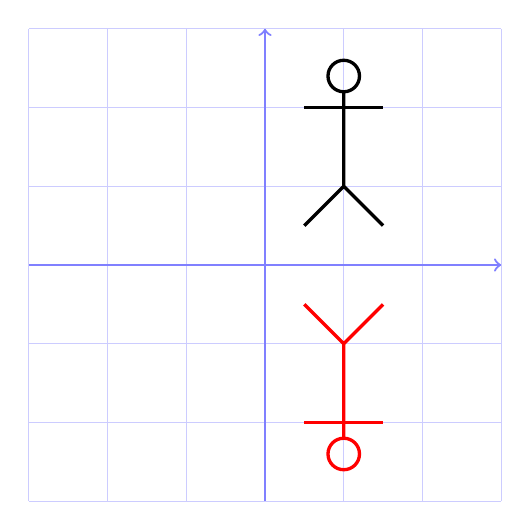
\begin{tikzpicture}
			\draw[blue!20!white] (-3,-3) grid (3,3);
			\draw[blue!50!white,->,thick] (0,-3) -- (0,3);
			\draw[blue!50!white,->,thick] (-3,0) -- (3,0);
			\draw[very thick] (0.5,0.5) -- (1,1) -- (1,2.2) -- (1,1) -- (1.5,0.5);
			\draw[very thick] (0.5,2) -- (1.5,2);
			\draw[very thick] (1,2.4) circle (0.2);
			\draw[red, very thick] (0.5,-0.5) -- (1,-1) -- (1,-2.2) -- (1,-1) -- (1.5,-0.5);
			\draw[red, very thick] (0.5,-2) -- (1.5,-2);
			\draw[red, very thick] (1,-2.4) circle (0.2);
		\end{tikzpicture}
		\end{center} 
	
		\begin{enumerate}
			\item die Identische Abbildung $ x \mapsto x $ auf der Geraden $ \lin(e_1) =\K \times \{ 0 \} $ und
			\item die Spiegelung $ x \mapsto -x $ auf der Geraden $ \lin(e_2) = \{ 0 \} \times \K $.
		\end{enumerate}
		
		Diese Abbildung des Raums $\K^2$ ist also eine \textquote{Zusammensetzung} von zwei linearen Abbildungen von eindimensionalen Räumen. Mit anderen Worten: die Abbildung schickt $e_1$ auf $e_1$ und $e_2$ auf $-e_2$. Die Abbildung ist durch diese Vorgabe eindeutig beschrieben, da eine lineare Abbildung durch die Angabe ihrer Wirkung auf einer Basis eindeutig festgelegt ist. Da $e_1$ auf $e_1$ geschickt wird, fällt man bei der Anwendung der Abbildung auf den Vektoren aus der Geraden $\lin(e_1)$ nicht aus dieser Geraden aus. Ebenso fällt man nicht aus der Geraden $\lin(e_2)$ aus. 
	\item
		Ein weiteres ähnliches Beispiel ist die Projektion $ x = (x_1,x_2) \mapsto (x_1,0) $ auf die $x_1$-Achse in $ \K^2 $. Diese zerfällt in 
		\begin{enumerate}
			\item Die identische Abbildung $ x \mapsto x $ auf der $x_1$-Achse$ \lin(e_1)= \K \times \{ 0 \} $ und
			\item Die Nullabbildung $ x \mapsto 0 $ auf der $x_2$-Achse $\lin(e_2)= \{ 0 \} \times \K $.
		\end{enumerate}
			\begin{center}
		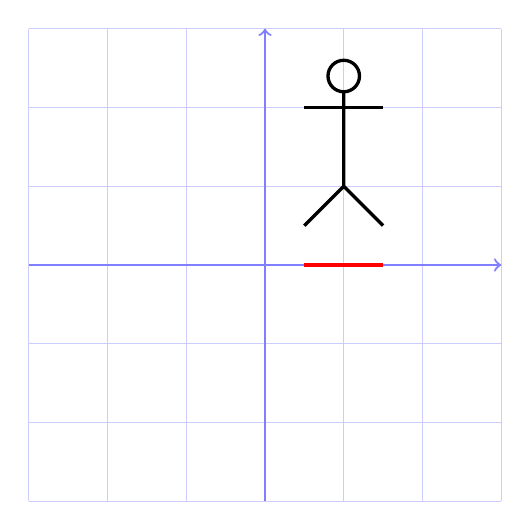
\begin{tikzpicture}
		\draw[blue!20!white] (-3,-3) grid (3,3);
		\draw[blue!50!white,->,thick] (0,-3) -- (0,3);
		\draw[blue!50!white,->,thick] (-3,0) -- (3,0);
		\draw[very thick] (0.5,0.5) -- (1,1) -- (1,2.2) -- (1,1) -- (1.5,0.5);
		\draw[very thick] (0.5,2) -- (1.5,2);
		\draw[very thick] (1,2.4) circle (0.2);
		\draw[red, very thick] (0.5,0) -- ( 1.5,0);
		\end{tikzpicture}
	\end{center} 
	
	\item Bei den vorigen beiden Abbildungen war die Zerlegung direkt erkennbar, weil die zugrundeliegenden Untervektorräume von $\K^2$ Koordinatenachsen waren. Hier noch ein Beispiel, in dem man ebenfalls eine Zerlegung findet, aber nicht bzgl. der Koordinaten Achsen. 
		Wir betrachten die Abbildung $ x = (x_1,x_2) \mapsto (x_2,x_1) $ auf $ \K^2 $. Diese Abbildung ist wie auch das erste Beispiel ebenfalls eine Spiegelung.
		\begin{enumerate}
			\item $ x \mapsto x $ auf der Geraden $ \{ (x_1,x_2) \in \K^2 : x_1 = x_2 \} $ und
			\item $ x \mapsto -x $ auf der Geraden $ \{ (x_1,x_2) \in \K^2 : x_1 = - x_2 \} $.
		\end{enumerate}
			\begin{center}
	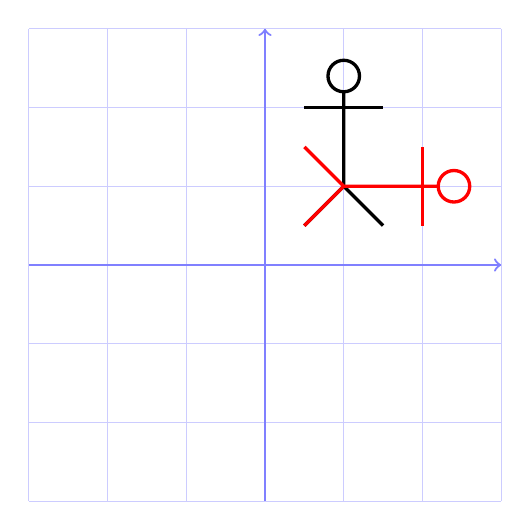
\begin{tikzpicture}
	\draw[blue!20!white] (-3,-3) grid (3,3);
	\draw[blue!50!white,->,thick] (0,-3) -- (0,3);
	\draw[blue!50!white,->,thick] (-3,0) -- (3,0);
	\draw[very thick] (0.5,0.5) -- (1,1) -- (1,2.2) -- (1,1) -- (1.5,0.5);
	\draw[very thick] (0.5,2) -- (1.5,2);
	\draw[very thick] (1,2.4) circle (0.2);
	\draw[red,very thick] (0.5,0.5) -- (1,1) -- (2.2,1) -- (1,1) -- (0.5,1.5);
	\draw[red,very thick] (2,0.5) -- (2,1.5);
	\draw[red,very thick] (2.4,1) circle (0.2);
	\end{tikzpicture}
	\end{center}

	\item
		Nun betrachten wir ein Links-Shift der Koordinaten $ (x_1,x_2) \mapsto (x_2,0) $ auf $ \K^2 $.
		Die Vektoren in der $x_1$-Achse bleiben nach der Anwendung der Abbildung in der $x_1$-Achse, denn sie werden auf $0$ abgebildet: 
		$ x \mapsto 0 $ auf $ \lin(e_1) = \K \times \{ 0 \} $. 
		Man findet aber keinen einen anderen eindimeinsionalen Untervektorraum von $\K^2$ mit der Eigenschaft, dass die Vektoren dieses Untervektorraums nach der Anwendung der Abbildung im fixierten Untervektorraum bleiben. 
		Diese Abbildung lässt sich also nicht als Zusammensetzung von Abbildungen eindimensionaler Untervektorräume darstellen. 
\end{enumerate}

\subsubsection{Definition von Eigenwerten und Eigenvektoren}

Nun haben wir genug Motivation für die Begriffe Eigenwert und Eigenvektor. 
Sei $ V $ Vektorraum über $ \K $ und sei $ F : V \to V $ lineare Abbildung. Ein Paar $(\lambda,v)$ aus einem Skalar $\lambda \in \K$  und einem Nichtnullvektor $ v \in V \setminus \{ 0 \} $ mit der Eigenschaft
\begin{equation}
	F(v) = \lambda v
\end{equation}
heißt \emph{Eigenpaar} von $F$. Dabei heißt $\lambda$ \emph{Eigenwert} von $F$ und $v$ \emph{Eigenvektor} zum Eigenwert $\lambda$ von $F$. 

Sie können nun Beispiele aus \ref{motiv:eigenwerte} nochmals betrachten und alle Eigenpaare der in \ref{motiv:eigenwerte} angegebenen linearen Abbildungen finden. Wenn wir in einem Eigenpaar $(\lambda,v)$ den Eigenvektor $v$ mit einem Nichtnullwert $\alpha \in \K \setminus \{0\}$ multiplizieren, so erhalten wir ein Eigenpaar $(\lambda, \alpha v)$, das sich im Wesentlichen von dem ursprünglichen Eigenpaar $(\lambda,v)$ nicht unterscheidet. Mit anderen Worten ist nur die Richtung eines Eigenvektors wichtig. Die genaue Skalierung des Eigenvektors des spielt keine Rolle. 

Analog werden diese Begriffe Eigenpaar, Eigenwert und Eigenvektor für eine quadratische Matrix eingeführt. Die Eigenwerte, Eigenvektoren und Eigenpaare von $ A \in \K^{n \times n} $ sind jene der zugehörigen Abbildung $ x \mapsto Ax $, oder ausformuliert: $(\lambda,v)$ mit $\lambda \in \K$ und $v \in \K^n \setminus \{0\}$ ist \emph{Eigenpaar} von $A$, wenn die Bedingung $A v = \lambda v$ erfüllt ist. 

\begin{bem}
Wie bereits in Teil~1 des Kurses erwähnt ermöglichen Matrizen eine konkrete Beschreibung der linearen Abbildung im ``konkreten Raum'' $\K^n$. Da man im Raum $\K^n$ die Standardbasis $e_1,\ldots,e_n$ hat, ist es naheliegend die Wirkung einer Abbildung des Raums $\K^n$ genau in dieser Basis festzuliegen. Genau dass macht die Matrix $A$ der Abbildung $x \mapsto A x$. Die Standardbasis ist aber nicht notwendigerweise eine Basis, in der man die zugrundeliegende Abbildung am besten versteht. Das ist einer der Gründe, warum der abstrakte Zugang zur linearen Algebra durch allgemeine Vektorräume $V$ günstig ist: man legt keine feste Basis fest. Des Weiteren muss man noch bedenken, dass nicht jeder Vektorraum eine Standardbasis hat. Tatsächlich hat zum Beispiel die Ebene $ E:= \{ (x,y,z) \, :\, x + 2 y - 3 z = 0 \} \subseteq \R^3$ keine Standardbasis, man kann aber stets eine Basis $b_1, b_2$ wählen und danach diese Ebene als $\R^2$ behandeln. Man kann z.B. eine $90$-Grad Drehung $ F: E \to E$ in der Ebene $E$ betrachten und analysieren. Wenn wir die lineare Algebra ausschließlich konkret auf der Basis von Vektoren aus $\K^n$ und Matrizen entwickelt hätten, hätten wir keine Sprache zur Verfügung zur Einführung und der Behandlung der Drehung $F$ wie oben. 
\end{bem}

\begin{bem}
	Es ist klar, dass der Begriff vom Kern
	$\ker(F)$ einer linearen Abbildung $F : V \to V$ mit Eigenvektoren zusammenhängt. Nichtnullvektoren aus dem Kern sind genau die Eigenwerte von $F$ zum Eigenwert $0$. 
\end{bem}

\begin{bem}
Ein Eigenvektor $v$ zum Eigenwert $1$ hat die Eigenschaft $F(v) = v$, das heißt, $v$ ist ein sogenannter Fixpunkt der Abbildung $v$. Solche Fixpunkte sind oft von einem besonderen Interesse. Der Vektor der Google-Pageranks der Internetseiten ist ein Fixpunkt einer linearen Abbildung, die durch die Vernetzung der Internetzung der Internetseiten bestimmt ist.
\end{bem}

\begin{bem}
Die Aufgaben $A x = b$ (Lösung von linearen Gleichungssystemen) und $A v = \lambda v$ (Eigenwertaufgabe) sind die zwei Grund-Rechenaufgaben der linearen Algebra. In der Numerik werden Sie verschiedene Methoden zur Lösung dieser zwei Aufgaben lernen. Die beiden Aufgaben sind nämlich der Hauptgegenstand der Numerischen Linearen Algebra. 

Hierbei wählt man $\C$ als den zugrundeliegenden Körper und führt die Berechnungen in der Praxis annähernd mit Hilfe der sogenannten Gleitkommazahlen.  Die Aufgabe $A v = \lambda v$ kann etwas konkreter in verschiedenen Varianten gestellt werden. In der numerischen Mathematik interessiert man sich oft für den Eigenwert $\lambda$ mit dem höchsten Betrag und einen zugehörigen Eigenvektor. Alle Rechenaufgaben aus der linearen Algebra, die wir bis jetzt betrachtet haben, konnten wir durch das Gauß-Verfahren (bzw. eine Variation davon) lösen. Die Eigenwertaufgabe ist aber die Aufgabe, bei der das Gauß-Verfahren \textbf{nicht} direkt hilft (man braucht weitere Ideen). Die Aufgabe ist eigentlich nicht linear, denn $\lambda$ ist unbekannt, $v$ ist ebenfalls unbekannt und die Aufgabe $A v = \lambda v$ enthält das \textbf{Produkt} dieser unbekannten Objekte. Sobald man das Unbekannte $v$ oder $\lambda$ bestimmt hat, ist man im Wesentlichen durch. Kennt man das $v$, so ermittelt man $\lambda$ als Streckungsfaktor der parallelen Vektoren $A v$ und $v$. Hat man $\lambda$ ermittelt, so reduziert sich die Bestimmung eines zugehörigen Eigenvektors zur Lösung des LGS $A v= \lambda v$ für einen unbekannten Vektor $v$.
\end{bem}

%\begin{bem}
%	Die Schwingung einer Feder ohne Dämpfung wird durch die lineare Differentialgleichung $m x''(t) + k x(t) = 0$ ($m$ Masse, $k$ die Federkonstante) die Startbedingungen beschrieben. Zu dieser Gleichung kann man die lineare Abbildung betrachten, welche der Funktion $x(t)$ die Funktion $m x''(t) + k x(t)$ zuordnet. Die Eigenwerte dieser lineare Abbildung heißen die Eigenfrequenzen. Bei $m=k=1$ hat man zum Bespiele die Lineare Abbildung $ x(t) \mapsto x''(t) + x(t)$. 
%\end{bem}

\subsubsection{Diagonalisierbarkeit von linearen Abbildungen}

Hier und im Folgenden sei $n \in \N$.
Sei $ V $ ein $ n $-dimensionaler Vektorraum über $ \K $. Eine Abbildung $ F \in \Lin(V) $ heißt diagonalisierbar, wenn eine Basis $ \mathcal{B} $ von $ V $ existiert, für welche die Matrix $ F_\mathcal{B} $ diagonal ist. Die Diagonalisierbaren Abbildungen sind die einfachsten Abbildungen in der Theorie der Eigenwerte und Eigenvektoren. 

Die nachfolgende Proposition formuliert Diagonalisierbarkeit in der Sprache der Eigenwerte und Eigenvektoren. 

\begin{propn}
	Sei $ V $ ein $ n $-dimensionaler Vektorraum und sei $ F \in \Lin(V) $. Dann sind die folgenden Bedingungen äquivalent:
	\begin{enumerate}
		\item
			$ F $ ist diagonalisierbar.
		\item
			$ V $ besitzt eine Basis aus Eigenvektoren von $ F $.
	\end{enumerate}
\end{propn}
\begin{proof}
	Um diese Proposition herzuleiten, reicht es aus, die Definition von $F_\mathcal{B}$ auszuschreiben. Die Matrix $F_\mathcal{B}$ der Abbildung $F$ bzgl. der Basis $\mathcal{B} = (b_1,\ldots,b_n)$ entsteht folgendermaßen: man wenden $F$ zu den Basisvektoren $b_1,\ldots,b_n$ und schreibt das Ergebnis jedes mal wieder in der Basis $b_1,\ldots,b_n$ auf. Die $i$-te Spalte enthält die Darstellung von $F(b_i)$ in der Basis $b_1,\ldots,b_n$. Die Eigenschaft, dass $F_\mathcal{B}$ diagonal mit Diagonalelementen $\lambda_1,\ldots,\lambda_n$ ist, bedeutet als, dass $f(b_i) = \lambda_i b_i$ erfüllst. Das heißt, $\mathcal{B}$ ist Basis aus Eigenvektoren von $F$, und die jeweiligen Diagonalelemente sind die entsprechenden Eigenwerte.
\end{proof}

\begin{bsp}[aus 6.1.1]
	Sei $ F(x_1,x_2) = (x_2,x_1) $. Dann ist $ b_1 = (1,1) $ Eigenvektor zum Eigenwert 1, $ b_2 = (-1,1) $ Eigenvektor zum Eigenwert -1 und $ \mathcal{B} = (b_1, b_2) $ eine Basis von $ \Q^2 $. D.h.
	\begin{equation*}
		F_\mathcal{B} = \begin{pmatrix}
			1 & 0 \\
			0 & -1
		\end{pmatrix}
	\end{equation*}
\end{bsp}
\begin{bsp}[aus 6.1.1]
	Sei $ F(x_1,x_2) = (x_2,0) $. Dies ist ein Beispiel einer ``problematischen'' Abbildung, welche man nicht diagonalisieren kann. Zeigen wir das durch ein Widerspruchsargument. Angenommen, $F$ hätte eine Basis $b_1,b_2$ aus Eigenvektoren mit den jeweiligen Eigenwerten $\lambda_1$ und $\lambda_2$. Die zweifache Anwendung von $F$ zu einem beliebigen Vektor aus $\K^2$ ergibt null ( $(x_1,x_2) \mapsto (x_2,0) \mapsto (0,0)$ ). Das heißt $F^2(x) =0$ für alle $x$. Wir haben aber $F(b_i) = \lambda_i b_i$ und somit $F^2(b_i) = F(\lambda_i b_i) = \lambda_i F(b_i) = \lambda_i^2 b_i$. Also ist $\lambda_i^2 b_i = 0$. Da $b_i$ kein Nullvektor ist, folgt $\lambda_i^2 = 0$. Daraus folgt $\lambda_i =0$. Wir haben $\lambda_1 = \lambda_2 = 0$. Unser Abbildung schickt somit den Basisvektor $b_i$ auf den Vektor $0 b_i =0$. Somit ist $F$ eine Nullabbildung, das widerspricht aber zu $F(e_2) = e_1 \ne 0$.
\end{bsp}

Durch die vorigen Beispiele sehen wir, dass man unproblematische (diagonalisierbare) sowie problematische (nichtdiagonalisierbare) Abbildungen hat. Wir sind an der Theorie interessiert, die uns helfen würde, die beiden Fälle auseinanderzuhalten. Im Rest des Kapitels werden Werkzeuge dazu entwickelt. 

Im Rest dieses Abschnitts besprechen wir noch  kurz die Diagonalisierbarkeit von quadratischen Matrizen. Eine Matrix $ A \in \K^{n \times n} $ heißt diagonalisierbar, wenn die lineare Abbildung $ x \mapsto Ax $ auf $ \K^n $ diagonalisierbar ist, 
mit anderen Worten: $ \K^n $ besitzt eine Basis $ b_1, \ldots, b_n $ mit $ Ab_i = \lambda_ib_i \enspace\forall i \in \is{1}{n} $, wobei $ \lambda_1, \ldots, \lambda_n \in \K $. Aus dieser Definition wird deutlich, dass die Eigenschaft von der Wahl des Körpers abhängig ist. Eine Matrix $A \in \R^{n \times n}$ ist auch eine Matrix aus $\C^{n \times n}$. Es gibt Fälle, in den $A$ bzgl. $\R$ nicht diagonalisierbar ist, aber bzgl. des größeren Körpers $\C$ diagonalisierbar. Mehr dazu später. 


\begin{propn}
	Sei $ A \in \K^{n \times n} $. Die Matrix $ A $ ist genau dann diagonalisierbar (bzgl. $\K$), wenn eine invertierbare Matrix $ B \in \K^{n \times n} $ existiert, sodass $ B^{-1}AB $ diagonal ist.
\end{propn}
\begin{proof}
	Wie der vorige Beweis brauchen wir auch hier, lediglich die Diagonalisierbarkeit in eine andere Sprache zu übersetzen, und zwar in die Sprache der Matrizen. 
	Sei $ A $ diagonalisierbar, d.h. es existiert eine Basis $ b_1, \ldots, b_n $ von $ \K^n $ mit $ Ab_i = \lambda_ib_i \enspace\forall i \in \is{1}{n} $, wobei $ \lambda_1, \ldots, \lambda_n \in \K $. Sei $ B = (b_1, \ldots, b_n) $. Dann ist
	\begin{equation*}
		A \begin{pmatrix}
			| && | \\
			b_1 & \cdots & b_n \\
			| && |
		\end{pmatrix} = \begin{pmatrix}
			| && | \\
			\lambda_1b_1 & \cdots & \lambda_nb_n \\
			| && |
		\end{pmatrix} = \begin{pmatrix}
			| && | \\
			b_1 & \cdots & b_n \\
			| && |
		\end{pmatrix} \begin{pmatrix}
			\lambda_1 && \\
			& \ddots & \\
			&& \lambda_n
		\end{pmatrix}
	\end{equation*}
	$ B $ ist invertierbar, weil die Spalten von $ B $ eine Basis bilden (vgl. LA I). Wir multiplizieren die vorige Gleichung mit $ B^{-1} $ von links und erhalten
	\begin{equation}
		B^{-1}AB = \begin{pmatrix}
			\lambda_1 && \\
			& \ddots & \\
			&& \lambda_n
		\end{pmatrix}
		\label{eq:6_1_3}
	\end{equation}
	Umgekehrt: sei $ B \in \K^{n \times n} $ eine invertierbare Matrix, für welche $ B^{-1}AB $ diagonal ist, d.h. \eqref{eq:6_1_3} gilt mit $ \lambda_1, \ldots, \lambda_n \in \K $. Es folgt: $ b_1, \ldots, b_n $ ist eine Basis von $ \K^n $ mit $ Ab_i = \lambda_ib_i \enspace\forall i \in \is{1}{n} $.
\end{proof}

\noindent Motiviert durch die vorige Proposition führen wir den Begriff der Ähnlichkeit von Matrizen ein. Matrix $ A \in \K^{n \times n} $ und $ \widetilde{A} \in \K^{n \times n} $ heißen \emph{ähnlich}, wenn eine invertierbare Matrix $ B \in \K^{n \times n} $ existiert mit $ B^{-1}AB = \widetilde{A} $.
Die Ähnlichkeit von Matrizen ist eine Äquivalenzrelation (Zeigen Sie das). 

\begin{bsp}
	$ \widetilde{A} = \begin{pmatrix}
		1 & 0 \\
		0 & -1
	\end{pmatrix}, A = \begin{pmatrix}
		0 & 1 \\
		1 & 0
	\end{pmatrix} \in \Q^2 $. Seien $ b_1 = \begin{pmatrix}
		1 \\ 1
	\end{pmatrix}, b_2 = \begin{pmatrix}
		1 \\ -1
	\end{pmatrix} $. Dann ist $ Ab_1 = b_1 $, $ Ab_2 = -b_2 $. D.h. für $ B = (b_1, b_2) $ ist $ AB = B\widetilde{A} \Leftrightarrow B^{-1}AB = \widetilde{A} $. Die Matrix $\widetilde{A}$ beschreibt eine Spiegelung an der $x_2$-Achse, die Matrix $A$ eine Spiegelung an der Achse $x_1=x_2$. Die Matrizen machen also tatsächlich was Ähnliches. 
\end{bsp}

In Bezug auf die Theorie der Eigenwerte und Eigenvektoren unterscheiden sich zwei verschiedene ähnliche Matrizen voneinander nicht (d.h., sie haben komplett die gleichen Eigenschaften in dieser Theorie).

\subsubsection{Diagonalisierbarkeit: eine hinreichende Bedingung}
\label{sec:6_1_4}

Wir diskutieren hier eine Bedingung, die in vielen Situationen hilft, Diagonalisierbarkeit zu erkennen. Bei der Diagonalisierung geht es um die Suche nach einer Basis, in der die Abbildung diagonal ist. Die Vektoren der Basis sollen Eigenvektoren sein. Wir sind als auf der Suche nach linear unabhängigen Eigenvektoren. Das folgende Lemma zeigt, dass wir im Fall von verschiedenen Eigenwerten, die lineare Unabhängigkeit geschenkt bekommen. 

\begin{lm}
	Sei $F: V \to V$ lineare Abbildung über einem Vektorraum $V$ und
	seien $ (\lambda_1,v_1), \ldots, (\lambda_m,v_m) $ Eigenpaare von $ F $ mit der Eigenschaft, dass $ \lambda_1, \ldots, \lambda_m $ \emph{paarweise verschieden} sind. Dann sind $ v_1, \ldots, v_m $ linear unabhängig.
\end{lm}
\begin{proof}
	Induktion über $ m \in \N $. Für $ m = 1 $ ist die Behauptung trivial. Angenommen, die Behauptung gilt für $ m-1 $ Eigenpaare mit $m \ge 2$. Wir betrachten nun $m$ Eigenpaare mit $m$ verschiedenen Eigenwerten. Seien $ \alpha_1, \ldots, \alpha_m \in \K $ beliebige Skalare mit
	\begin{equation}
		\alpha_1v_1 + \ldots + \alpha_mv_m = 0
		\label{eq:6_1_4}
	\end{equation}
	Wir multiplizieren \eqref{eq:6_1_4} mit $ \lambda_m $ und erhalten:
	\begin{equation*}
		\lambda_m\alpha_1v_1 + \ldots + \lambda_m\alpha_{m-1}v_{m-1} + \lambda_m\alpha_mv_m = 0
	\end{equation*}
	Die Anwendung von $ F $ zu \eqref{eq:6_1_4} ergibt:
	\begin{equation*}
		\lambda_1\alpha_1v_1 + \ldots + \lambda_m\alpha_mv_m = 0
	\end{equation*}
	In der Differenz der vorigen zwei Gleichungen verschwindet der Term mi $v_m$:
	\begin{equation*}
		(\lambda_1 - \lambda_m)\alpha_1v_1 + \ldots + (\lambda_{m-1} - \lambda_m)\alpha_{m-1}v_{m-1} = 0
	\end{equation*}
	% 04.05.2015
	Nach Induktionsvoraussetzung sind $ v_1, \ldots, v_{m-1} $ linear unabhängig. Also folgt aus der vorigen Gleichung, dass alle Koeffizienten der linearen Kombination auf der linken Seite gleich $0$ sind:
	\begin{equation*}
		(\lambda_1 - \lambda_m)\alpha_1 = \ldots = (\lambda_{m-1} - \lambda_m)\alpha_{m-1} = 0
	\end{equation*}
	Da die Eigenwerte paarweise verschieden sind, ist $ \lambda_i - \lambda_m \neq 0 $ für alle $ i \in \is{1}{m-1} $,l erhält man
	\begin{equation*}
		\alpha_1 = \ldots = \alpha_{m-1} = 0
	\end{equation*}
	Das Einsetzen in \eqref{eq:6_1_4} ergibt $ \alpha_m v_m = 0 $. Mit $ v_m \neq 0 $ folgt $ \alpha_m = 0 $. Wir haben aus \eqref{eq:6_1_4} $\alpha_1 = \cdots = \alpha_m =0$ erhalten. D.h., $ v_1, \ldots, v_m $ sind linear unabhängig.
\end{proof}

\begin{thm} 
	Sei $ F : V \to V$ lineare Abbildung eines $n$-dimensionalen Vektorraums $V$, welche $n$ paarweise verschiedene Eigenwerte $ \lambda_1, \ldots, \lambda_n \in \K$ besitzt. Dann ist $ F $ diagonalisierbar.
\end{thm}
\begin{proof}
	Das vorige Lemma ergibt, dass die Eigenvektoren $b_1,\ldots,b_n$ zu den Eigenwerten $\lambda_1,\ldots,\lambda_n$ eine Basis von $V$ bilden. Die Matrix von $F$ bzgl. dieser Basis ist diagonal. 
\end{proof}

Wann ist eine hinreichende Bedingung für eine gewünschte Eigenschaft nützlich? In der Regel wünscht man sich eine möglichst allgemeine hinreichende Bedingung, also eine Bedingung, die nicht zu restriktiv ist. Aus dieser Perspektive ist die oben präsentierte hinreichende Bedingung der Diagonalisierbarkeit zumindest bzgl. des Körpers der komplexen Zahlen \textbf{sehr} nützlich.  Denn diese Bedingung ist bzgl. $\C$ generisch erfüllt: wenn Sie etwa eine Matrix $A$ aus $\C^{n \times n}$ generieren, in dem Sie die $n^2$ Komponenten von $A$ aus einem Bereich, etwa aus dem Segment $[-1,1]$ gleichmäßig und unabhängig ziehen, dann kriegen Sie mit Wahrscheinlichkeit $1$ eine Matrix mit $n$ paarweise verschiedenen Eigenwerte in $\C$. ``Generisch erfüllt'' ist aber nicht nicht das selbe wie (bedingungslos) ``erfüllt''. Wenn sie zwei unabhängige gleichmäßig verteilte Werte $x,y$ aus $[0,1]$ ziehen, dann ist die Eigenschaft $x \ne y$ generisch erfüllt (es ist also unwahrscheinlich, dass $x=y$ gilt). Es gibt zwar Werte $x,y \in [0,1]$ mit $x =y$, diese Werte bilden eine eindimensionale Ausnahme im Quadrat aller Paare $(x,y) \in [0,1]^2$. 


\subsubsection{Eigenraum}

Alle Eigenwerte zu einem festen Eigenwert plus der Nullvektor bilden einen Untervektorraum, den sogenannten Eigenraum. Sei $F: V \to V$ lineare Abbildung eines Vektorraums $V$ und sei $\lambda \in \K$. Dann heißt
\begin{equation}
	\Eig(F,\lambda) := \{ v \in V : F(v) = \lambda v \}
\end{equation}
der \emph{Eigenraum} von $ F $ bzgl. $ \lambda $. Wir setzen in dieser Definition nicht voraus, dass $\lambda$ Eigenwert von $F$ ist. Wenn $\lambda$ kein Eigenwert ist, dann enthält $\Eig(F,\lambda)$ nichts außer dem Nullvektor. Fassen wir die Grundeigenschaften der Eigenräume zusammen: 

\begin{propn}
	Für eine lineare Abbildung $F : V \to V$ eines Vektorraums $V$ und ein $\lambda \in V$ gilt: 
	\begin{enumerate}
		\item
			$ \Eig(F,\lambda) $ ist Untervektorraum von $ V $.
		\item
			$ \lambda $ ist genau dann Eigenwert von $ F $, wenn $ \Eig(F,\lambda) \neq \{ 0 \} $ gilt.
		\item
			Wenn $ \lambda $ Eigenwert von $ F $ ist, dann gilt für $ v \in V $:
			
			$ v $ ist Eigenvektor von $ F $ zu $ \lambda \Longleftrightarrow v \in \Eig(F,\lambda) \setminus \{ 0 \} $
		\item
			$ \Eig(F,\lambda) = \ker(\lambda \id_V - F) $
		\item
			Wenn $ \lambda_1, \lambda_2 \in \K $ verschieden sind, dann gilt $ \Eig(F,\lambda_1) \cap \Eig(F,\lambda_2) = \{ 0 \} $.
	\end{enumerate}
\end{propn}
\begin{proof}
	(i) - (iv) klar, (v) folgt aus dem Lemma in \ref{sec:6_1_4} im Fall $ m = 2 $.
\end{proof}

Durch die Einführung von $\Eig(F,\lambda)$ und die Bemerkung $\Eig(F,\lambda) = \ker(\lambda \id - F)$ schaffen wir mehr Ordnung in unserer Diskussion der Eigenwerte und Eigenvektoren. Jedem Eigenwert $\lambda$ wird nun ein Vektorraum zugeordnet $\Eig(F,\lambda)$, in dem alle Eigenvektoren zu $\lambda$ enthalten sind und der als Kern der Abbildung $\lambda \id - F$ beschrieben werden kann. Wegen (v) gibt es paarweise keine ``Überlappungen'' der Räume $\Eig(F,\lambda)$ (bis auf den Nullvektor, der in jedem Vektorraum enthalten ist). 

\clearpage
\subsection{Das charakteristische Polynom}

Betrachten wir die Version der Eigenwertaufgabe, in der man \text{alle} Eigenwerte bestimmen möchte. Es stellt sich heraus, dass die Eigenwerte die Nullstellen eines besonderen Polynoms sind, das man einer Matrix bzw. einer linearen Abbildung zuordnet. Dieses Polynom wird das charakteristische Polynom genannt. Wenn man das charakteristische Polynome ausrechnen kann, so muss man dann ``nur noch'' die Nullstellen davon berechnen können. 

Am Anfang vom Teil~1 des Kurses haben wir uns kurz mit Polynomen beschäftigt. Hier eine kurze Zusammenfassung vom Wissen über Polynome, das wir in diesem Abschnitt benötigen:

\begin{tcolorbox}[title=Wiederholung]
	Sei $ t $ eine Unbestimmte.
	\begin{itemize}
		\item
			Der Polynomring $ \K[t] $ enthält die Monome $ t^0, t^1, t^2, t^3, \ldots $, wobei $ t^0 $ mit $ 1 $ aus $ \K $ identifiziert wird, und endliche Linearkombinationen dieser Monome mit Koeffizienten aus $ \K $. Das Polynom ist ein formaler Ausdruck (wird also durch die Angabe der Koeffizienten für seine Monome festgelegt).
		\item
			Addition und Multiplikation von Polynomen erfolgt komponentenweise.
		\item
			Die Gleichheit zweier Polynome aus $ \K[t] $ wird durch den Koeffizientenvergleich definiert.
		\item
			Ein Polynom $ f \in \K[t] $ kann an einem $ \lambda \in \K $ ausgewertet werden. Somit definiert jedes $ f \in \K[t] $ die Polynomfunktion $ \lambda \mapsto f(\lambda) $ auf $ \K $.
		\item Polynom ist nicht das gleiche wie Polynomfunktion. Nehmen wir als Beispiel den Körper $\K = \{0,1\}$. Die Polynome $f=t$ und $g=t^2$ in $\K[t]$ bestimmen die selbe Polynomfunktion (die identische Funktion), das sind aber trotzdem verschiedene Polynome. 
	\end{itemize}
\end{tcolorbox}

\subsubsection{Das charakteristische Polynom einer Matrix}

In Kapitel~\ref{Determinanten} über die Determinanten haben aus den Formeln für die Determinanten Formeln für Grundaufgaben der linearen Algebra hergeleitet. Nun sind die Eigenwerte dran, wir erstellen mit der Verwendung der Determinanten eine Gleichung für die Eigenwerte. 

\begin{propn}
	Sei $ A \in \K^{n \times n} $, $ \lambda \in \K $. Dann sind folgende Aussagen äquivalent:
	\begin{enumerate}
		\item
			$ \lambda $ ist Eigenwert von $ A $.
		\item
			$ \det(\lambda I - A) = 0 $.
	\end{enumerate}
\end{propn}
\begin{proof}
	$\lambda$ ist genau dann Eigenwert von $v$, wenn die Gleichung $A v = \lambda v$ eine Nichtnull-Lösung $v$ besitzt. Das bedeutet, dass der Kern der quadratischen Matrix $\lambda I - A$ ungleich Null ist. Das Letztere ist äquivalent zu $\det(\lambda I - A) =0$, wie wir aus dem Kapitel~\ref{Determinanten} über die Determinanten wissen. 
\end{proof}

\noindent Hier und im Folgenden sei $ t $ eine Unbestimmte. Motiviert durch die vorige Proposition möchten wir das charakteristische Polynom $ p_A \in \K[t] $ einer Matrix $ A \in \K^{n \times n} $ durch die Gleichung
\begin{equation} \label{p_A}
	p_A := \det(t I - A)
\end{equation}
einführen. Da wir mathematisch sauber arbeiten wollen, können wir das $p_A$ auf diese Weise  noch nicht bedenkenlos definieren. Schauen wir uns den Ausdruck $\det(t I - A)$ genauer an. $t I - A$ ist die Matrix, deren Komponenten zum Ring $\K[t]$ der Polynome gehören. Etwa im Fall $n=2$:
\[
	 \begin{pmatrix} a_{11} & a_{12} \\ a_{21} & a_{22} \end{pmatrix}  = \begin{pmatrix} t-a_{11} & -a_{12} \\ -a_{21} & t- a_{22} \end{pmatrix} 
\]
Wir betrachten also die Determinante einer Matrix, deren Komponenten zum kommutativen Ring $\K[t]$ gehören. Die Theorie der Determinanten haben wir aber für die Matrizen entwickelt, deren Elemente zu einem Körper gehören. Streng genommen können wir also von dieser Theorie ohne extra Begründung keinen Gebrauch machen. Es ist klar, dass man in die Leibniz-Formel auch Matrizen über einem Ring einsetzen kann, denn in der Leibniz-Formel wird nirgendwo dividiert (es reicht als aus, einen kommutativen Ring zu haben, in dem im Gegensatz zu einem Körper nicht jedes Element invertierbar sein muss). Also könnte man im Prinzip $p_A$ durch die Leibniz-Formel einführen. Aber, das wäre noch kein Ausweg. Denn wir wollen die Theorie der Determinanten benutzen, deren Gültigkeit wir nur im Fall von Matrizen über einem Körper verifiziert. Wir können die Situation ziemlich einfach retten: und zwar werden wir den Ring $\K[t]$ in einen Körper einbetten. 

\subsubsection{Rechtfertigung der Definition vom charakteristischen Polynom}

Es ist lehrreich einen Vergleich mit den ganzen Zahlen zu machen. Von einer Matrix mit ganzzahligen Komponenten $A \in \Z^{n \times n}$ können wir die Determinante berechnen, da der Ring $\Z$ der ganzen Zahlen zum Körper $\Q$ rationaler Zahlen erweitert werden kann. Also gehört $A  \in \Z^{n \times n}$ zu $\Q^{n \times n}$ und somit hat $A$ die Determinante bzgl. des Körpers der rationalen Zahlen. Diese Determinante kann unter anderem durch die Leibniz-Formel berechnet werden, in der nicht dividiert wird. Das zeigt also, das die Determinante einer ganzzahligen Matrix eine ganze Zahl ist.  Obwohl wir die rationalen Zahlen als Hilfstruktur benutzt haben, ist unsere Eingabe $A \in \Z^{n \times n}$ sowie Rückgabe $\det(A)$ ganzzahlig. 


In der Theorie der Ringe und Körper gibt es eine Verallgemeinerung der Konstruktion der rationalen Zahlen aus den ganzen Zahlen. Auf Basis welcher kommutative Ringe $R$ kann man Quotienten $\frac{a}{b}$ mit $a,b \in R$ und $b \ne 0$ einführen? Wenn der Ring $R$ Nullteiler hat, hat man ein Problem. Nehmen wir etwa an, $a$ und $b$ sind zwei Elemente von einem kommutativen Ring $R$ mit eins, die nicht gleich null sind und deren Produkt $a b$ gleich null ist (in $\Z / 6 \Z$ sind es zum Beispiel die Restklassen von $2$ und $3$). Die Quotienten können wir in einem solchen Ring nicht sinnvoll einführen. Im Prinzip könnten wir $\frac{1}{a}$ und $\frac{1}{b}$ betrachten, weil die Nenner ungleich null sind, wenn wir aber die beiden Quotienten multiplizieren  kriegen wir ein Problem: $\frac{1}{a} \cdot \frac{1}{b} = \frac{1}{a b} = \frac{1}{ 0}$. Im Ring der ganzen Zahlen hat man keine Nullteiler, daher lassen sich die Quotienten (also die rationalen Zahlen) korrekt einführen. 

Genau so hat man auch im Polynomring $\K[t]$ keine Nullteiler, und somit hat man auch eine wohldefinierte Weise die Quotienten $\frac{f}{g}$ von Polynomen $f, g \in \K[t]$ mit $g \ne 0$ einzuführen. Die Menge solcher Quotienten, ausgestattet mit den natürlichen Operationen $+$ und $\cdot$, bildet den sogenannten Quotientenkörper $\K(t)$. Es ist keine Überraschung, dass die Addition und Multiplikation folgendermaßen eingeführt werden: 
\begin{align}
\frac{f_1}{g_1} + \frac{f_2}{g_2} &:= \frac{f_1g_2 + f_2g_1}{g_1g_2} \\
\frac{f_1}{g_1} \cdot \frac{f_2}{g_2} &:= \frac{f_1f_2}{g_1g_2}
\end{align}
Des Weiteren lässt sich ein und der selbe Quotient auf mehrere Weisen hinschreiben. Wir müssen also klären, wann zwei Quotienten gleich sind. Hier auch keine Überraschungen: 
\begin{equation}
\frac{f_1}{g_1} = \frac{f_2}{g_2} \quad\Leftrightarrow\quad f_1g_2 = f_2g_1.
\end{equation}
Die Konstruktion des Quotientenkörper kann natürlich auch noch formaler beschrieben werden: ein Quotient ist eine Äquivalenzklasse aus Paaren (Zähler,Nenner) (mit Zähler aus $\K[t]$ und Nenner aus $\K[t] \setminus \{0\}$),  wobei zwei solche Paare $(f_1,g_1)$ und $(f_2, g_2)$ äquivalent sind, wenn $f_1 g_2 = f_2 g_1$ gilt. Sie können sich gerne überlegen, dass die oben angeführten Konstruktionen mathematisch korrekt sind: die eingeführte Relation ist tatsächlich eine Äquivalenzrelation, $+$ und $\cdot$ sind unabhängig davon, durch wie man den Quotienten konkret dargestellt und $\K(t)$ ist tatsächlich ein Körper. 

Der Ring $\K[t]$ wird als Unterstruktur von $\K(t)$ aufgefasst, denn $f \in \K[t]$ wird natürlicherweise mit dem Quotienten $\frac{f}{1}$ identifiziert. 

Nun hat unser Definition des charakteristischen Polynoms $\K[t]$ eine eindeutige Interpretation. Man hat
\[
	p_A := \det ( t I - A).
\]
Die Elemente der Matrix $t I - A$ gehören zum Ring $\K[t]$ und somit auch zum Körper $\K(t)$ der rationalen Funktionen. Somit wissen wir dass $\det(t I - A)$ bzgl. des Körpers $\K(t)$ definiert. Aber aus der Leibniz-Formel (in der nicht dividiert wird) wissen wir, dass $\det( t I - A)$ zum Ring $\K[t]$ gehört.

\begin{bem} \hfill {\normalfont 08.05.2015} \\
	Zur Berechnung von charakteristischen Polynomen können jede Methode aus dem Kapitel~5 benutzen: Leibniz-Formel, Laplace-Entwicklung, Gauß-Verfahren bzgl. des Körpers $ \K(t) $.
\end{bem}

\begin{bsp}
	Hier einige Beispiele der charakteristischen Polynome: 
	\begin{center}
	\begin{tabular}{c|c}
		Matrix & Das charakteristische Polynom \\
		\hline
		$ \begin{pmatrix}
			0 & 0 \\ 0 & 0
		\end{pmatrix} $ & $ \det\begin{pmatrix}
			t & 0 \\ 0 & t
		\end{pmatrix} = t^2 $ \\
		$ \begin{pmatrix}
			0 & 1 \\ 0 & 0
		\end{pmatrix} $ & $ \det\begin{pmatrix}
			t & 1 \\ 0 & t
		\end{pmatrix} = t^2 $ \\
		$ \begin{pmatrix}
			1 & 0 \\ 0 & 0
		\end{pmatrix} $ & $ \det\begin{pmatrix}
			t - 1 & 0 \\ 0 & t
		\end{pmatrix} = (t-1)t = t^2 - t $ \\
		$ \begin{pmatrix}
			1 & 1 \\ 0 & 1
		\end{pmatrix} $ & $ \det\begin{pmatrix}
			t-1 & -1 \\ 0 & t-1
		\end{pmatrix} = (t-1)^2 $ \\
		$ \begin{pmatrix}
			1 & 1 \\ 1 & 1
		\end{pmatrix} $ & $ \det\begin{pmatrix}
			t-1 & -1 \\ -1 & t-1
		\end{pmatrix} = (t-1)^2 - 1 = t(t-2) $ \\
	\end{tabular}
	\end{center}
\end{bsp}

\begin{bem}
	Ist $R$ ein kommutativer Ring mit $1$ und ohne Nullteiler, so ist bildet die Menge der Quotienten $\frac{a}{b}$ mit $a \in R$ und $b \in \R \setminus \{0\}$, zusammen mit $+$ und $\cdot$ (die genauso wie oben eingeführt werden), den sogenannten Quotientenkörper $\operatorname{Quot}(R)$ des Rings $R$. Anhand dieses Körpers kann man die Determinanten der Matrizen aus $R^{n \times n}$ einführen. 
\end{bem}

\subsubsection{Nullstellen, Grad und Koeffizienten des charakteristischen Polynoms}

\begin{propn}
	Sei $ A \in \K^{n \times n} $ mit $ n \in \N $ und $ \lambda \in \K $. Dann sind die folgenden Aussagen äquivalent:
	\begin{enumerate}
		\item
			$ \lambda $ ist Eigenwert von $ A $.
		\item
			$ \lambda $ ist Nullstelle von $ p_A $, d.h. $ p_A(\lambda) = 0 $.
	\end{enumerate}
\end{propn}
\begin{proof}
	Die Aussage ist nichts anders als eine Umformulierung von Proposition aus 6.2.1 ($ \lambda $ Eigenwert von $ A \Leftrightarrow \det(\lambda I - A) = 0 $).
\end{proof}


\begin{bsp}
	Im charakteristischen Polynom sind alle Eigenwerte als seine Nullstellen gespeichert. Das Polynom enthält aber noch mehr Information über die Matrix.  
	
	Betrachten wir den binären Körper $ \K = \{0,1\}$. Hier zwei Matrizen: 
	\begin{align*}
		 A & = \begin{pmatrix}
		0 & 0 & 0 \\
		1 & 0 & 1 \\
		0 & 1 & 1
	\end{pmatrix} \in \K^{3 \times 3}, 
	&
	O & = \begin{pmatrix}
		0 & 0 & 0 \\
		0 & 0 & 0 \\
		0 & 0 & 0
	\end{pmatrix} \in \K^{3 \times 3}. 
	\end{align*}
	Diese Matrizen sind schon sehr grundlegend unterschiedlich, denn keine Matrix ist ähnlich zur Nullmatrix (im buchstäblichen Sinne der Definition der Ähnlichkeit). 
	
	Berechnen wir die charakteristischen Polynome der beiden Matrizen (man beachte, dass im binären Körper $-1=1$ gilt): 
	\begin{align*}
		p_A &= \det\begin{pmatrix}
			t & 0 & 0 \\
			1 & t & 1 \\
			0 & 1 & t+1
		\end{pmatrix} = t^2(t+1) + t = t^3 + t^2 + t = t(t^2 + t + 1) \\
		p_O &= \det\begin{pmatrix}
				t & 0 & 0 \\
				0 & t & 0 \\
				0 & 0 & t
			\end{pmatrix} = t^3
	\end{align*}
	Die beiden Polynome sind nur einer Stelle Null: an der Null. Das heißt, die beiden Matrizen haben einen einzigen Eigenwert: den Null. Anhang der Eigenwerte sind also die Matrizen nicht unterscheidbar. Auch anhand der Auswertung des charakteristischen Polynoms an den Werten aus $\K$ nicht: $p_A(0) = p_O(0) = 0$ und $p_A(1) = p_O(1) = 1$. Aber $p_A$ und $p_O$ sind zwei verschiedene Polynome. Wir erkennen also den Unterschied von $A$ und $O$ an den charakteristischen Polynomen in diesem Fall. 
\end{bsp}

Welche Informationen sind im charakteristischen Polynom als Koeffizienten enthalten? Zwei interessanten Koeffizienten sind die Koeffizienten der Monome $t^0$ und $t^{n-1}$: 

\begin{propn}
	Sei $ A = (a_{ij})_{i,j=1,\ldots,n} \in \K^{n \times n} $. Dann hat das charakteristische Polynom die Form 
	\[
		p_A = t^n - (a_{11} + \cdots + a_{nn}) t^{n-1} + \cdots + (-1)^n \det(A),
	\]
	d.h., der Koeffizient vom Monom $t^n$ ist $1$, der Koeffizient vom Monom $t^{n-1}$ ist $- (a_{11} + \cdots + a_{nn})$, und der Koeffizient vom Monom $t^0$ ist $(-1)^n \det(A)$. 
\end{propn}
\begin{proof}
	Der Koeffizient vor $ t^0 $ ist $ p_A(0) = \det(0 \cdot I - A) = \det(-A) = (-1)^n \det(A) $. 
	
	Nach der Leibniz-Formel gilt:
	\begin{equation*}
		p_A = \det(tI-A) = \sum_{\sigma \in S_n} \sign(\sigma) \underbrace{\prod_{i=1}^n (t \delta_{i,\sigma(i)} - a_{i,\sigma(i)})}_{=:f_\sigma}
	\end{equation*}
	%{\mathclap{\begin{minipage}{0.3\textwidth}
%	Dieses Produkt ist genau dann ein Polynom vom Grad $ n $, wenn $ i = \sigma(i) \enspace\forall i $, d.h. wenn $ \sigma = \id $.
%\end{minipage}}}
	Beim Polynom $f_\sigma$ trägt jedes $i$ mit $\sigma(i)=i$ ein Faktor $t - a_{ii}$ bei. Die Faktoren zu $i$ mit $\sigma(i) \ne i$ sind Konstanten. Somit ist der Grad von $f_\sigma$ gleich der Anzahl der Fixpunkte von $\sigma$, das sind die Indizes $i$ mit $\sigma(i) =i$. Die identische Permutation hat $n$ Fixpunkte, alle anderen weniger als $n-1$. Daraus folgt, dass die Koeffizienten von $p_A$ bei den Monomen $t^n$ und $t^{n-1}$ die gleichen sind wie beim Polynom $f_{\sigma} = (t -a_{11}) \cdots (t - a_{nn})$ zur identischen Permutation $\sigma$. Das ergibt die gewünschten Ausdrücke für die Koeffizienten der Monome $t^n$ und $t^{n-1}$. 
\end{proof}

\noindent Den Wert $\tr(A):= a_{11} + \ldots + a_{nn} $ nennt man die \emph{Spur} der Matrix $ A = (a_{ij}) \in \K^{n \times n} $  (die Bezeichnung stammt vom englischen Wort \textquote{trace}). Wir habe also 
\[
	p_A = t^n - \tr(A) t^{n-1} + \cdots + (-1)^n \det(A). 
\]
Durch das charakteristische Polynom erkennt man also die Spur sowie die Determinante von $A$. 

\subsubsection{Das charakteristische Polynom, die Determinante und die Spur von linearen Abbildungen}

Ähnliche Matrizen haben das gleiche charakteristische Polynom: 

\begin{lm}
	Seien $ A, \widetilde{A} \in \K^{n \times n} $ ähnliche Matrizen. Dann haben $ A $ und $ \widetilde{A} $ das gleiche charakteristische Polynome. Des Weiteren sind die Determinante und die Spur von $A$ und $\widetilde{A}$ gleich. 
\end{lm}
\begin{proof}
	Laut der Definition der Ähnlichkeit gilt  $ \widetilde{A} = B^{-1}AB $ für eine invertierbare Matrix $ B \in \K^{n \times n} $. 
	Es reicht, die Behauptung über das charakteristische Polynom zu zeigen, denn die Informationen über die Determinante und die Spur ist in den Koeffizienten des charakteristischen Polynoms enthalten. Die Gleichheit der charakteristischen Polynome wird direkt verifiziert: 
	\begin{align*}
		p_{\widetilde{A}} &= 
		 \det(tI - \widetilde{A}) 
		\\ &= \det(tI - B^{-1}AB)
		 \\
		&= \det(tB^{-1}IB - B^{-1}AB) 
		\\ &= \det(B^{-1}(tI - A)B) 
		\\
		&= \det(B^{-1}) \det(tI - A) \det(B) 
		\\ &= \det(tI - A) = p_A \qedhere
	\end{align*}
\end{proof}

%\begin{klr}
%	Sei $F : V \to V$ lineare Abbildung eines $n$-dimensionalen Vektorraums und seien $\A$ und $\B$ Basen von $V$. 
%\end{klr}

 Sei $ V $ ein $ n $-dimensionaler Vektorraum über $ \K $ mit $ n \in \N $. Sei $ F \in \Lin(V) $. Aus dem vorigen Lemma folgt, dass für zwei beliebige Basen $ \A $ und $ \B $ von $ V $ die Matrizen $ F_\A $ und $ F_\B $ das gleiche charakteristische Polynom, die gleiche Determinante und die gleich Spur haben (vgl. den Abschnitt über den Basiswechsel aus LA I: $ F_\A = T_{\A \gets \B} F_\B T_{\B \gets \A} $ mit $ T_{\A \gets \B}T_{\B \gets \A} = I $, denn $ F_\A $ und $ F_\B $ sind ähnlich). \\[10pt]
%
D.h. wir können $ \det(F) $, $ \tr(F) $ und $ p_F $ (das charakteristische Polynom von $ F $) als
\begin{equation}
	\begin{aligned}
		\det(F) &:= \det(F_\B) \\
		\tr(F) &:= \tr(F_\B) \\
		p_F &:= p_{F_\B}
	\end{aligned}
\end{equation}
definieren, wobei die rechten Seiten von der Basis $ \B $ von $ V $ unabhängig sind.

\subsubsection{Der Satz von Cayley-Hamilton}


In ein Polynom $ f = \sum_{i=0}^{d} c_it^i \in \K[t] $ kann man nicht nur Werte, sondern auch kompliziertere Objekte wie z.B. quadratische Matrizen einsetzen. Wir definieren die Auswertung $ f(A) $ von $f$ an einer Matrix $A \in \K^{n \times n}$ als 
\[
	 f(A) := \sum_{i=0}^{d} c_i A^i.
\]

Für $ f = t^2 - t + 1 $ erhält man z.B. $ f(A) = A^2 - A^1 + A^0 = A^2 - A + I $.

\begin{bem}
Die Menge $ \K[A] = \{ p(A) : p \in \K[t] \} $ ist ein kommutativer Ring mit 1, wenn wir $\K[A]$ mit der Addition und Multiplikation von Matrizen ausstatten. Der Ring $\K[A]$ `lebt' innerhalb des Rings $\K^{n \times n}$. Im Gegenteil zu $\K[A]$ ist $\K^{n \times n}$ aber für alle $n \ge 2$ nicht kommutativ. Dass $\K[A]$ kommutativ ist, lässt sich direkt prüfen: das liegt daran, dass $A^i A^j = A^j A^i$ für alle $i, j \in \N_0$ erfüllt ist, denn die linke und die rechte Seite sind gleich $A^{i+j}$.   
\end{bem} 

\begin{bsp}
	Hier einige Beispiele von Formeln, die in $\K[A]$ gelten: 
	\begin{align*}
			(A + I)^2 & = A^2 + 2 A + I
			\\ (A+I)(A-I) & = A^2 - I
			\\ (A + I)^3 &= A^3 + 3 A^2 + 3 A + I
			\\ (A- I) (A^2 + A + I) & = A^3 - I
	\end{align*}
	Wenn man die Matrix $A$ durch eine Zahl ersetzt und $I$ durch die Zahl $1$, so erhält man die bekannte Formeln aus der Schule, die man durch das Ausmultiplizieren herleiten kann. Auch die hier angegebenen Formeln können durch Ausmultiplizieren hergeleitet werden.  Die oben präsentierten $4$ Formeln gelten für eine beliebige Matrix $A$. Es gibt natürlich auch Formeln, die für konkrete Matrizen spezifisch sind. Zum Beispiel gilt $A^2 = I$ wenn $x \mapsto A x$ eine Spiegelung ist (an einem Punkt oder an einer Ebene oder noch allgemeiner) und es gilt $A^2 = A$ wenn $A$ eine Projektion ist (auf eine ebene auf eine Gerade...)
\end{bsp} 

\begin{bem}
	Interessanterweise ist $\K[A]$ nicht nur einfach ein kommutativer Ring mit $1$, die Struktur von $\K[A]$ ist sogar noch etwas reichhaltiger. Es ist nämlich klar, dass $\K[A]$ auch ein Vektorraum ist: $\K[A]$ ist Untervektorraum des Vektorraums $\K^{n \times n}$, was man direkt verifizieren kann. Einen Ring mit einer kompatiblen Vektorraum nennt man eine Algebra. $\K[A]$ ist eine Algebra über dem Körper $\K$. 	
\end{bem}

\begin{bem}
	Wenn man einen neuen (endlich-dimensionalen) Vektorraum entdeckt bzw. einführt, dann ist eine der ersten quantitativen Fragen, die man stellen kann ist: was ist die Dimension? Wir können also auch im Fall von $\K[A]$ fragen: 
	was ist die Dimension von $\K[A]$? Das wissen wir zwar noch nicht, aber wir können zumindest eine erste Abschätzung machen: $\K[A]$ ist Untervektorraum von $\K^{n \times n}$, daher kann die Dimension von $\K[A]$ nicht höher als $\dim( \K^{n \times n}) = n^2$ sein. Wir werden in Kürze feststellen, dass der genau wert deutlich kleiner ist. 
\end{bem} 

Wenn eine Formel oder eine Aussage einfach formulierbar oder verblüffend ist, so merkt man sie am leichtesten. Der Satz von Cayley-Hamilton ist sehr einfach formuliert \emph{und} sehr verblüffend!

\begin{thm}[Der Satz von Cayley-Hamilton für Matrizen]
	Sei $ A \in \K^{n \times n} $. Dann gilt:
	\begin{equation}
		p_A(A) = 0.
	\end{equation}
\end{thm}

Nochmals mit Worten: wenn wir in das charakteristische Polynome einer Matrix die Matrix selbst einsetzen, kriegen wir die Null-Matrix. 

Ein pragmatischer Mensch würde vielleicht fragen: \emph{wieso} tun wir das denn? Es gibt verschiedene Anwendungen. Bevor wir aber sie diskutieren, wollen wir aber zuerst den Satz beweisen. 

\begin{proof}
	Wir werden mit den Komponenten von $A$ arbeiten. Sei also $ A = (a_{ij}) \in \K^{n \times n} $. Des Weiteren sei $ B(t) = (b_{ij}(t)) \in \K[t]^{n \times n} $ die komplementäre Matrix von $ (tI - A)^\top $. Dass wir $t I - A$ ins Spiel bringen, ist logisch, denn $p_A$ ist die Determinante von $t I -A$, und unsere Behauptung involviert $p_A$. Man beachte aber, dass wir $t I - A$ transponiert haben. 
	
	Aus den Grundeigenschaften der komplementären Matrizen erhalten wir die Gleichungen 
	\begin{equation*}
		\sum_{j=1}^n b_{ij}(t) (t \delta_{jk} - a_{kj}) = \det(tI - A) \cdot \delta_{ik}
	\end{equation*}
	für alle $ i,k \in \is{1}{n} $. Die Gleichungen enthalten das charakteristische Polynom $p_A = \det(t I - A)$ auf der rechte Seiten. Der Plan ist nun, in die aufgestellten polynomiellen Gleichungen die Matrix $A$ an der Stelle der Unbestimmten $t$ einzusetzen. Durch das Einsetzen erhalten wir
	\begin{equation*}
		\sum_{j=1}^{n} b_{ij}(A) \cdot (\delta_{jk}A - a_{kj}I) = p_A(A)\delta_{ik}
	\end{equation*}
	Multipliziere nun von rechts mit $ e_k $:
	\begin{equation*}
		\sum_{j=1}^{n} b_{ij}(A) \cdot \underbrace{(\delta_{jk}A - a_{kj}I) e_k}_{\delta_{jk}Ae_k - a_{kj}e_k} = p_A(A)\delta_{ik} e_k
	\end{equation*}
	und summiere über $ k \in \is{1}{n} $:
	\begin{align}
		\label{cayley:hamilton:aufloesung} 
		\sum_{k=1}^{n} \sum_{j=1}^{n} b_{ij}(A) \cdot (\delta_{jk}Ae_k - a_{kj}e_k) &= p_A(A) \sum_{k=1}^{n} \delta_{ik} e_k 
	\end{align}
	Uns bleibt es, die linke und die rechte Seite der letzten Gleichung zu vereinfachen. $\delta_{ik}$ ist nur für $i=k$ gleich $1$ und ansonsten gleich $0$. Daher ist die rechte Seite gleich $p_A(A) e_i$. Die linke Seite von \eqref{cayley:hamilton:aufloesung} sieht etwas umständlich aus kann aber deutlich vereinfacht werden. Wir verändern die Reihenfolge der beiden Summe und erhalten dann
	\begin{align*}
		\sum_{j=1}^{n} b_{ij}(A) \cdot \Bigg(
		\underbrace{\sum_{k=1}^{n} \delta_{jk}Ae_k}_{Ae_j} -
		\underbrace{\sum_{k=1}^{n} a_{kj}e_k}_{Ae_j}
		\Bigg) = 0.
	\end{align*}
	Also ist $p_A(A) e_i = 0$ für alle $i$. Folglich ist $p_A(A)$ die $n \times n$ Null-Matrix. 
\end{proof}

\begin{bsp}
	Der Satz von Cayley-Hamilton ist sehr allgemein. Allgemeine Aussagen können  manchmal überwältigend sein. In solchen Situationen kann es helfen, konkrete Beispiele zur allgemeinen Aussage zu betrachten. Betrachten wir die Matrix der Drehung um einen Winkel $\varphi$ am Ursprung. Hier die Zusammenfassung, wie die Matrix aussieht und wie Sie auf Standardbasisvektoren wirkt: 
	\begin{figure}[H]
		\centering
		\begin{minipage}{0.35\textwidth}
			\centering
			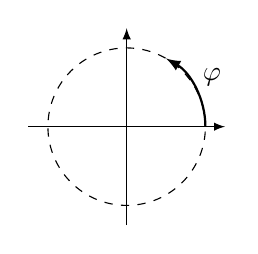
\begin{tikzpicture}
	\draw[-latex] (-1.25,0) -- (1.25,0);
	\draw[-latex] (0,-1.25) -- (0,1.25);
	\draw[dashed] (0,0) circle (1);
	\draw[thick,-latex] (1,0) arc (0:60:1);
	\node at (30:1.25) {$ \varphi $};
\end{tikzpicture}
		\end{minipage}
		\begin{minipage}{0.55\textwidth}
			\centering
			$ \begin{aligned}
				e_1 &\mapsto \begin{pmatrix} \cos \varphi \\ \sin \varphi \end{pmatrix} 
				\\ 
				e_2 &\mapsto \begin{pmatrix} -\sin \varphi \\ \cos \varphi \end{pmatrix} \\
				A &= \begin{pmatrix}
					\cos \varphi & -\sin \varphi \\
					\sin \varphi & \cos \varphi
				\end{pmatrix}
			\end{aligned} $
		\end{minipage}
	\end{figure}
	\noindent $ A^2 $ dreht einen Vektor um $ 2\varphi $. Demnach ist $ A^2 = \begin{pmatrix}
		\cos 2\varphi & -\sin 2\varphi \\
		\sin 2\varphi & \cos 2\varphi
	\end{pmatrix} $. Außerdem gilt:
	\begin{align*}
		p_A &= \det \begin{pmatrix}
			t - \cos \varphi & \sin \varphi \\
			-\sin \varphi & t - \cos \varphi
		\end{pmatrix} \\
		&= t^2 - 2t \cos \varphi + \cos^2 \varphi + \sin^2 \varphi \\
		&= t^2 - 2t \cos \varphi + 1
	\end{align*}
	Nach Cayley-Hamilton ist $ A^2 - 2 \cos \varphi \cdot A + I = 0 $, d.h.
	\begin{equation*}
		\begin{pmatrix}
			\cos 2\varphi & -\sin 2\varphi \\
			\sin 2\varphi & \cos 2\varphi
		\end{pmatrix} = 2 \cos \varphi \begin{pmatrix}
			\cos \varphi & -\sin \varphi \\
			\sin \varphi & \cos \varphi
		\end{pmatrix} - \begin{pmatrix}
			1 & 0 \\
			0 & 1
		\end{pmatrix}
	\end{equation*}
	Demzufolge ist 
	\[
		 \cos(2\varphi) = 2 \cos^2 \varphi - 1 
	\]
		und 
	\[ 
		\sin(2\varphi) = 2\sin\varphi\cos\varphi . 
	\]
	Das sind die bekannten Formeln für den Kosinus und Sinus des doppelten Winkels. Es kann sein, dass Sie diese Formeln bereits in der Schule hatten (in Mathematik oder Physik). Diese Formeln haben wir aus dem Satz von Cayley-Hamilton hergeleitet. Es gibt natürlich auch andere, direktere Möglichkeiten, die beiden Formeln herzuleiten. Uns geht in diesem Beispiel darum, das neue Wissen, das wir gerade erwerben mit dem alten Wissen zu verbinden (je mehr Verbindungen sehen wir, desto besser verstehen wir den Stoff). 
	
	Können wir auch Formeln für den Kosinus und Sinus des dreifachen Winkel herleiten? Der dreifache Winkeln hängt mit $A^3$ zusammen. Wir müssen also herausfinden, wie $A^3$ von $A$ abhängt. Wir wissen bereits, dass $A^2 =  2 \cos \varphi \, A - I$ gilt. Daher ist $A^3= A \cdot A^2 = A( 2 \cos \varphi A - I ) =   2 \cos \varphi A^2 - A $. Und dann können wir für $A^2$ den Ausdruck $2 \cos \varphi \, A - I $ noch einmal einsetzen. Das ergibt: 
	\[
		A^3 = 2 \cos \varphi (2 \cos \varphi A - I )= (4 \cos^2 \varphi -1) A - 2 \cos \varphi  I. 
	\]
	Wenn man nun die letzte Formel Komponentenweise ausschreibt sieh  man, wie man $\cos 3 \varphi$ und $\sin 3 \varphi$ mit Hilfe von $\cos \varphi$ und $\sin \varphi$ darstellen kann.
\end{bsp}

\begin{bem}
	Durch Cayley-Hamilton wird $ A^n $ ($ A \in \K^{n \times n} $) als Linearkombination von $ A^0, \ldots, A^{n-1} $ dargestellt. Man kann hierdurch die Potenzen $ A^k $ mit Hilfe der Multiplikation von Polynomen ausrechnen (vgl. Beispiel oben). Cayley-Hamilton hilft uns also im Ring $\K[A]$ zu rechnen. 
\end{bem}

\begin{bem}
	Sei $ A \in \K^{n \times n} $. Als Vektorraum über $ \K $ hat $ \K[A] $ die Dimension höchstens $ n $. (Übungsaufgabe)
\end{bem}

\begin{bem}
	Wir können verschiedene interessante algebraische Strukturen als $\K[A]$ umsetzen. Die Algebra $\K[A]$ ist also oft eine konkrete Matrix-basierte `Umsetzung' einer abstrakten algebraischen Struktur. Natürlich hat man auch die Verbindung in die andere Richtung: denn jede quadratische Matrix $A$ wird mit  der Algebra $\K[A]$ in Verbindung gesetzt.  Somit wird $A$ ein Element der Algebraischen Struktur $\K[A]$. 
\end{bem}

Quadratische Matrizen sind konkrete Analoga der linearen Abbildungen eines Vektorraums $V$. Wir können natürlich auch eine lineare Abbildung $F : V \to V$ in ein Polynom 
$ p = \sum_{i=1}^{d} c_it^i \in \K[t] $ einsetzen: wir definieren $p(F)$ als $ p(F) = \sum_{i=0}^{d} c_iF^i $. Auch in diesem Fall wird der Ring $ \K[F] := \set{q(F) : q \in \K[t]} $ eingeführt. Der Ring $\K[F]$ ist auch ein Untervektorraum von $\Lin(V)$. 

In der Sprache der linearen Abbildungen wird der Satz von Cayley-Hamilton folgendermaßen formuliert: 

\begin{thm}[Satz von Cayley-Hamilton für lineare Abbildungen]
	Sei $ V $ endlichdimensionaler Vektorraum und $ F : V \to V $ lineare Abbildung. Dann gilt:
	\begin{equation}
		p_F(F) = 0
	\end{equation}
\end{thm}
\begin{proof}
	Übungsaufgabe.
\end{proof}

\clearpage
\subsection{Diagonalisierbarkeit}

\subsubsection{Eine notwendige und eine hinreichende Bedingung}

Sei $ f \in \K[t] \setminus \set{0} $. $ f $ \emph{zerfällt in Linearfaktoren}, wenn $ f $ als $ f = c(t-\mu_1) \cdots (t-\mu_n) $ mit $ c \in \K \setminus \set{0} $ und $ \mu_1, \ldots, \mu_n \in \K $ darstellbar ist. Diese Eigenschaft ist von der Wahl von $ \K $ abhängig.

\begin{bspe}\
	\begin{enumerate}
		\item
			$ f = 3t^2-6t+3 \in \K[t] $ zerfällt für $ \K = \Q $ in Linearfaktoren, denn es ist \\
			$ f = 3(t-1)^2 $ ($ c=3 $ und $ \mu_1=\mu_2=1 $).
		\item
			$ f = t^2 - 2 \in \K[t] $ zerfällt für $ \K = \Q $ nicht in Linearfaktoren, aber bzgl. $ \K = \R $: \\
			$ f = (t-\sqrt{2})(t+\sqrt{2}) $.
	\end{enumerate}
\end{bspe}

\begin{thm}
	Sei $ V $ Vektorraum über $ \K $ mit $ \dim(V) = n \in \N $. Sei $ F \in \Lin(V) $. Dann gilt:
	\begin{enumerate}
		\item
			Ist $ F $ diagonalisierbar, so zerfällt $ p_F $ in Linearfaktoren.
		\item
			Ist $ p_F = (t-\mu_1) \cdots (t-\mu_n) $ mit paarweise verschiedenen $ \mu_1, \ldots, \mu_k \in \K $, d.h. $ p_F $ zerfällt in Linearfaktoren und hat $ n $ paarweise verschiedene Nullstellen, dann ist $ F $ diagonalisierbar.
	\end{enumerate}
\end{thm}
\begin{proof}\
	\begin{enumerate}
		\item
			Sei $ F $ diagonalisierbar, d.h. es existiert eine Basis $ \B $ von $ V $, für welche die Matrix $ F_\B $ diagonal ist.
			
			D.h. $ F_\B = \diag(\mu_1, \ldots, \mu_n) $ mit $ \mu_1, \ldots, \mu_n \in \K $ und es gilt $ p_F = p_{F_\B} = \det(tI - F_\B) = (t-\mu_1) \cdots (t-\mu_n) $. Also zerfällt $ p_F $ in Linearfaktoren.
		\item
			$ \mu_1, \ldots, \mu_n $ sind paarweise verschiedene Eigenwerte von $ F $. Aus Theorem \ref{sec:6_1_4} ergibt sich die Behauptung. \qedhere
	\end{enumerate}
\end{proof}

\subsubsection{Vielfachheit von Nullstellen und Zerlegbarkeit in Linearfaktoren}

\begin{propn}
	Sei $ f \in \K[t] \setminus \{ 0 \} $ und sei $ \lambda \in \K $ Nullstelle von $ f $. Dann existiert eine durch $ f $ und $ \lambda $ eindeutig bestimmte Zahl $ r \in \N $ und ein Polynom $ g \in \K[t] \setminus \{ 0 \} $ mit $ f = (t - \lambda)^r g $ und $ g(\lambda) \neq 0 $.
\end{propn}
\begin{proof}
	Aufgabe.
\end{proof}
\noindent Die Zahl $ r $ aus der vorigen Proposition nennt man die \emph{algebraische Vielfachheit} der Nullstelle $ \lambda $ von $ f $.
\begin{bem}
	$ r $ und $ g $ zu $ f $ lassen sich durch die iterative Verwendung der Polynomdivision bestimmen (vgl. Schule).
\end{bem}
\begin{propn}
	Sei $ f \in \K[t] \setminus \{ 0 \} $. Seien $ \lambda_1, \ldots, \lambda_k $ ($ k \in \N_0 $) die paarweise verschiedenen Nullstellen von $ f $. Dann kann $ f $ als das Produkt
	\begin{equation}
		f = (t - \lambda_1)^{r_1} \cdots (t - \lambda_k)^{r_k} g
		\label{eq:6_3_2}
	\end{equation}
	dargestellt werden, wobei $ r_1, \ldots, r_k \in \N $ mit $ g \in \K[t] \setminus \{ 0 \} $ keine Nullstellen in $ \K $ hat. Die vorige Darstellung ist bis auf die Nummerierung der Terme $ (t - \lambda_i)^{r_i} $ $ (i \in \is{1}{k}) $ eindeutig.
\end{propn}
\begin{proof}
	Aufgabe.
\end{proof}
\begin{bem}
	Die Darstellung \eqref{eq:6_3_2} lässt sich mit Hilfe der Polynomdivision bestimmen.
\end{bem}
\begin{bem}
	$ f $ zerfällt genau dann in Linearfaktoren, wenn in der Darstellung \eqref{eq:6_3_2} $ g $ eine Konstante ist, d.h. $ g \in \K \setminus \{ 0 \} $.
\end{bem}
\begin{bem}
	Zur Berechnung von \eqref{eq:6_3_2} muss die Menge $ \{ \lambda_1, \ldots, \lambda_k \} $ von $ f $ berechnet werden. Möglichkeiten dafür sind:
	\begin{enumerate}
		\item
			$ \K $ ist endlich $ \rightsquigarrow $ alle Elemente von $ \K $ durchprobieren (die direkte Methode).
		\item
			$ \K = \Q $. Man hat die folgende notwendige Bedingung. Sei $ f \in \Z[t] \setminus \{ 0 \} $ mit $ f = c_0 t^0 + \ldots + c_d t^d $ ($ c_0, \ldots, c_d \in \Z, c_d \neq 0, d \in \N $). Sei $ \lambda = \frac{a}{b} $ mit teilerfremden $ a,b \in \Z \setminus \{ 0 \} $ Nullstelle von $ f $, d.h. $ f(\lambda) = 0 $. Dann gilt:
			\begin{itemize}
				\item $ a $ teilt $ c_0 $
				\item $ b $ teilt $ c_d $
			\end{itemize}
			Dies sind wiederum endlich viele Möglichkeiten.
	\end{enumerate}
\end{bem}
%\clearpage
\begin{bspe}\
	\begin{enumerate}
		\item
			$ A = \begin{pmatrix}
				0 & 0 & 0 \\
				1 & 0 & 1 \\
				0 & 1 & 1
			\end{pmatrix} \in \K^{3 \times 3} $ mit $ \K = \Z/2\Z $. Dann ist
			
			$ p_A = \det\begin{pmatrix}
				t & 0 & 0 \\
				1 & t & 1 \\
				0 & 1 & t+1
			\end{pmatrix} = t^2(t+1) + t = t^3 + t^2 + t = t \underbrace{(t^2 + t + 1)}_{\mathclap{\text{\normalsize zerfällt nicht in Linearfaktoren}}} $.
			
			Es folgt: $ A $ ist nicht diagonalisierbar (bzgl. $ \K = \Z/2\Z $).
		\item
			$ A = \begin{pmatrix}
				0 & 0 & 0 \\
				1 & 0 & 1 \\
				0 & 1 & 1
			\end{pmatrix} \in \K^{3 \times 3} $ mit $ \K = \Q $. Dann ist
			
			$ p_A = \det\begin{pmatrix}
				t & 0 & 0 \\
				-1 & t & -1 \\
				0 & -1 & t-1
			\end{pmatrix} = t^2(t-1) - t = t^3 - t^2 - t = t\underbrace{(t^2 - t - 1)}_{\mathclap{\text{\normalsize hat keine Nullstellen in $ \Q $ }}} $.
			
			Es folgt: $ A $ ist bzgl. $ \K = \Q $ nicht diagonalisierbar.
		\item
			Sei $ A $ wie oben und $ \K = \R $. Man hat drei unterschiedliche Nullstellen: 0, $ \frac{1}{2} \pm \frac{\sqrt{5}}{2} $. D.h. $ p_A = t(t - \frac{1}{2} - \frac{\sqrt{5}}{2})(t - \frac{1}{2} + \frac{\sqrt{5}}{2}) $. Es folgt: $ A $ ist diagonalisierbar.
		\item
			Sei $ A = \begin{pmatrix}
				0 & -1 \\
				1 & 0
			\end{pmatrix} \in \K^{2 \times 2} $, $ \K=\R $.
			
			Es ist $ p_A = t^2 + 1 $. $ \lambda^2 + 1 \neq 0 \enspace \forall \lambda \in \R \Rightarrow $ bzgl. $ \K = \R $ zerfällt $ A $ nicht in Linearfaktoren.
		\item
			Sei $ A = \begin{pmatrix}
				0 & -1 \\
				1 & 0
			\end{pmatrix} \in \K^{2 \times 2} $, $ \K=\C $. Sei $ i $ die imaginäre Einheit, d.h. $ i^2 + 1 = 0 $.
			
			Es ist $ p_A = t^2 + 1 = (t-i)(t+i) $. $ \Rightarrow A $ ist diagonalisierbar.
		\item
			Sei $ A = O \in \K^{2 \times 2} $ und $ \K $ beliebig. Dann ist $ p_A = t^2 $. $ A $ ist diagonalisierbar (das Theorem aus 6.3.1 kann das aber nicht entscheiden).
		\item
			Sei $ A = \begin{pmatrix}
				0 & 1 \\
				0 & 0
			\end{pmatrix} \in \K^{2 \times 2} $ und $ \K $ beliebig. Dann ist $ p_A = t^2 $. $ A $ ist nicht diagonalisierbar (vgl. Kapitel 6...).
	\end{enumerate}
\end{bspe}

\subsubsection{Ungleichungen für die algebraische und die geometrische Vielfachheit}
\label{sec:6_3_3}

Sei $ V $ ein endlichdimensionaler Vektorraum über $ \K $ und sei $ F \in \Lin(V) $. Für die Diagonalisierbarkeit von $ F $ ist es notwendig, aber im allgemeinen Fall nicht hinreichend, dass $ p_F $ in Linearfaktoren zerfällt. Wir sind auf der Suche nach einer Bedingung an $ F $, die in Kombination mit der vorigen Bedingung an das charakteristische Polynom, die Diagonalisierbarkeit von $ F $ charakterisiert.

Sei $ \lambda $ Eigenwert von $ F $, d.h. $ p_F(\lambda) = 0 $. Die Vielfachheit von $ \lambda $ als Nullstelle von $ p_F $ nennt man die \emph{algebraische Vielfachheit} des Eigenwerts $ \lambda $ von $ F $.

Die Dimension von $ \Eig(F,\lambda) = \ker(F - \lambda \id) $ nennt man die \emph{geometrische Vielfachheit} des Eigenwerts $ \lambda $ von $ F $.

\begin{thm}
	Sei $ V $ $ n $-dimensionaler Vektorraum über $ \K $ mit $ n \in \N $ und sei $ F \in \Lin(V) $. Sei $ \lambda $ Eigenwert von $ F $. Sei $ k $ die geometrische Vielfachheit des Eigenwerts $ \lambda $ von $ F $ und $ l $ die algebraische Vielfachheit. Dann gilt: $ k \leq l $.
\end{thm}
\begin{proof}
	Sei $ b_1, \ldots, b_k $ eine Basis von $ \Eig(F,\lambda) = \{ v \in V : F(v) = \lambda v \} $. Wir erweitern $ b_1, \ldots, b_k $ zu einer Basis $ \B = (b_1, \ldots, b_n) $ von $ V $. Die Matrix $ F_\B $ hat die folgende Struktur:
	\begin{equation*}
		F_\B = \begin{pmatrix}
			\lambda I_k & C \\
			O & D
		\end{pmatrix}
	\end{equation*}
	mit $ C \in \K^{k \times (n-k)} $ und $ D \in \K^{(n-k) \times (n-k)} $. Es folgt: $ p_F = p_{F_\B} = \det(tI - F_\B) = \det((t - \lambda)I)_{k \times k}\det(tI - D)_{(n-k) \times (n-k)} = (t - \lambda)^k \det(tI - D) $. Es folgt, dass die algebraische Vielfachheit von $ l $ mindestens $ k $ ist.
\end{proof}

\subsubsection{Charakterisierung der Diagonalisierbarkeit}

\begin{thm}
	Sei $ V $ ein $ n $-dimensionaler Vektorraum über $ \K $ mit $ n \in \N $. Sei $ F \in \Lin(V) $. Dann sind die folgenden Bedingungen äquivalent:
	\begin{enumerate}
		\item
			$ F $ ist diagonalisierbar.
		\item
			Das charakteristische Polynom von $ F $ zerfällt in Linearfaktoren und für jeden Eigenwert $ \lambda $ von $ F $ sind die geometrische und die algebraische Vielfachheit von $ \lambda $ gleich.
		\item
			$ V $ ist direkte Summe der Eigenräume zu den Eigenwerten von $ F $.
	\end{enumerate}
\end{thm}
\begin{proof}\
	\begin{description}[font=\normalfont]
		\item[(i)$ \Rightarrow $(ii):]
			Sei $ F $ diagonalisierbar. Dann existiert eine Basis $ \B = (b_1, \ldots, b_n) $ und Werte $ \mu_1, \ldots, \mu_n \in \K $ mit $ F(b_i) = \mu_ib_i $ für alle $ i \in \is{1}{n} $. $ \Rightarrow $
			\begin{equation*}
				F_\B = \begin{pmatrix}
					\mu_1 && \\
					& \ddots & \\
					&& \mu_n
				\end{pmatrix}
				\quad\Rightarrow\quad
				p_F = p_{F_\B} = \det(tI - F_\B) = (t-\mu_1) \cdots (t-\mu_n),
			\end{equation*}
			also zerfällt $ p_F $ in Linearfaktoren. Sei $ \lambda $ beliebiger Eigenwert von $ F $ und sei $ r \in \K $ die algebraische Vielfachheit von $ \lambda $. Dann gilt $ \lambda = \mu_i $ für genau $ r $ unterschiedliche Indizes $ i \in \is{1}{n} $. O.B.d.A. sei $ \lambda = \mu_1 = \ldots = \mu_r $ und $ \lambda \neq \mu_i $ für $ i > r $. Somit sind $ b_1, \ldots, b_r $ linear unabhängige Eigenvektoren zu $ \lambda $, sodass die Ungleichung $ r = \dim(\lin(b_1, \ldots, b_r)) \leq \dim(\Eig(F,\lambda)) =: l $ erfüllt ist. Es folgt, dass die Gleichung $ r = l $ erfüllt ist, da die Ungleichung $ l \leq r $ in \ref*{sec:6_3_3} gezeigt wurde.
		\item[(ii)$ \Rightarrow $(iii):]
			Sei (ii) erfüllt. Seien $ \lambda_1, \ldots, \lambda_k $ ($ k \in \N $) die paarweise verschiedenen Nullstellen von $ p_F $. Wegen (ii) gilt $ p_F = (t-\lambda_1)^{r_1} \cdots (t-\lambda_k)^{r_k} $ mit $ r_1, \ldots, r_k \in \N $. Wegen (ii) gilt auch $ r_i = \dim(\Eig(F,\lambda_i)) $ für alle $ i \in \is{1}{n} $.
			
			Wir zeigen, dass die Summe der Räume $ \Eig(F,\lambda_i) $ mit $ i \in \is{1}{k} $ direkt ist. Seien $ v_i \in \Eig(F,\lambda_i) \enspace \forall i \in \is{1}{k} $ Vektoren mit $ v_1 + \ldots + v_k = 0 $. Da Eigenvektoren zu paarweise verschiedenen Eigenwerten linear unabhängig sind (Lemma \ref{sec:6_1_4}), folgt $ v_1 = \ldots = v_k = 0 $. Also ist die Summe der Räume $ \Eig(F,\lambda) $ mit $ i \in \is{1}{k} $ direkt. Für die Dimension dieser Summe gilt:
			\begin{align*}
				&\ \dim(\Eig(F,\lambda_1) \oplus \ldots \oplus \Eig(F,\lambda_k)) \\
				=&\ \dim(\Eig(F,\lambda_1)) + \ldots + \dim(\Eig(F,\lambda_k)) && \text{nach Theorem \ref{sec:3_6_4}} \\
				=&\ r_1 + \ldots + r_k && \text{wegen (ii)} \\
				=&\ n = \dim(V)
			\end{align*} %TODO: Formel aufhübschen!
			$ \Rightarrow \Eig(F,\lambda_1) \oplus \ldots \oplus \Eig(F,\lambda_k) = V $
		\item[(iii)$ \Rightarrow $(i):]
			Sei (iii) erfüllt und seien $ \lambda_1, \ldots, \lambda_k $ die Eigenwerte wie oben. Sei $ \B_i $ eine Basis von $ \Eig(F,\lambda_i) $ für $ i \in \is{1}{k} $. Wegen (iii) erhält man durch das Zusammenfügen der Systeme $ \B_1, \ldots, \B_k $ eine Basis $ \B $ von $ V $. Für diese Basis gilt
			\begin{equation*}
				F_\B = \begin{pmatrix}
					\lambda_1 I_{r_1} && \\
					& \ddots & \\
					&& \lambda_k I_{r_k}
				\end{pmatrix}
			\end{equation*}
			mit $ r_i = \dim(\Eig(F,\lambda_i)) \in \N \enspace \forall i \in \is{1}{k} $. Also ist $ F $ diagonalisierbar. \qedhere
	\end{description}
\end{proof}
\begin{bem}
	Das vorige Theorem zusammen mit Methoden zur Bestimmung von Nullstellen und Faktorisierung von Polynomen führt zu Rechenverfahren, welche die Diagonalisierbarkeit entscheiden können und gegebenenfalls eine Basis $ \B $ finden, für die $ F_\B $ diagonal ist:
	\begin{enumerate}[label=\arabic*.]
		\item Bestimme alle Eigenwerte der gegebenen Matrix und die jeweiligen algebraischen Vielfachheiten. 
		\item Berechne  zu jedem der Eigenwerte  eine Basis des Eigenraums (und somit auch die geometrische Vielfachheit). 
		\item Ist für einen der Eigenwerte die geometrische Vielfachheit ungleich der algebraischen Vielfachheit, dann ist die gegebene Matrix nicht diagonalisierbar. 
		\item Sonst ist die Matrix Diagonal in der Basis, die durch das Zusammenfügen der Basen der Eigenräume entsteht. 
	\end{enumerate} 
\end{bem}

\clearpage
\subsection{Die Jordansche Normalform}
\label{sec:6_4}

\subsubsection{Die Voraussetzungen}
\label{sec:6_4_1}

Das Hauptresultat dieses Abschnitts wird mit den folgenden Voraussetzungen formuliert.

\begin{tcolorbox}
	Sei $ V $ ein $ n $-dimensionaler Vektorraum über $ \K $ mit $ n \in \N $. Sei $ F \in \Lin(V) $ eine Abbildung, deren charakteristisches Polynom in Linearfaktoren zerfällt, d.h.
			\begin{equation*}
				p_F = (t - \lambda_1)^{r_1} \cdots (t - \lambda_k)^{r_k}
			\end{equation*}
			mit paarweise verschiedenen $ \lambda_1, \ldots, \lambda_k \in \K $ und $ r_1, \ldots, r_k \in \N $.
\end{tcolorbox}

\noindent Es sei daran erinnert, dass die vorige Voraussetzung im Fall $ \K = \C $ für jede lineare Abbildung $ F \in \Lin(V) $ erfüllt ist (im Gegenteil zum Fall $ \K = \R $).

\subsubsection{Das Ziel und der Ansatz}

Unter den Voraussetzungen aus \ref{sec:6_4_1} wollen wir eine Basis $ \B $ von $ V $ finden, für welche die Matrix $ F_\B $ möglichst wenig Nichtnullkomponenten außerhalb der Diagonalen hat (die genaue Struktur von $ F_\B $ wird später beschrieben).

Im allgemeinen Fall wird die gesuchte Basis $ \B $ nicht nur aus Vektoren der Eigenräume $ \Eig(F,\lambda_i) = \ker(F - \lambda_i \id) $ bestehen, sondern auch aus Vektoren der Räume $ \ker(F - \lambda_i \id)^2 $, $ \ker(F - \lambda_i \id)^3 $, usw. Beachte hier: wenn eine einfache Anwendung einer Abbildung einen Vektor nicht auf $0$ bringt, dann könnte es immer noch sein, dass eine zweifache oder eine dreifache Anwendung den Vektor auf $0$ bringt. Mit anderen Worten wird der Kern der Potenz einer linearen Abbildung im Allgemeinen größer, wenn der Exponent wächst. 

Wenn ein Vektor $ v \in \ker(F - \lambda_i \id) \setminus \{ 0 \} $ in $ \B $ aufgenommen wird, so hat $ F_\B $ bzgl. des Vektors $v$ die Struktur
\begin{equation*}
	F_\B = \bordermatrix{
		& && \bordernote{v} && \cr
		& \tikz[na] \node[coordinate] (6_4_2_n1) {};\hspace{0.5cm} && 0 & \tikz[na] \node[coordinate] (6_4_2_n3) {};\hspace{0.5cm} & \cr
		& && \vdots && \cr
		& && 0 && \cr
		\bordernote{v} & && \lambda_i && \cr
		& && 0 && \cr
		& && \vdots && \cr
		& & \ \tikz[na] \node[coordinate] (6_4_2_n2) {}; & 0 && \ \tikz[na] \node[coordinate] (6_4_2_n4) {}; \cr
	},
	\begin{tikzpicture}[remember picture, overlay]
		\draw[pattern=north east lines,draw=gray,pattern color=gray] (6_4_2_n1) rectangle (6_4_2_n2);
		\draw[pattern=north east lines,draw=gray,pattern color=gray] (6_4_2_n3) rectangle (6_4_2_n4);
	\end{tikzpicture}
\end{equation*}
denn $v$ ist Eigenvektor von $F$ zum Eigenwert $\lambda_i$, sodass man $F(v) = \lambda_i v$ hat. 

Was passiert, wenn man nicht genug Eigenvektoren hat um eine Basis daraus zu bilden? 
Wenn etwa ein Vektor $ w \in \ker(F - \lambda_i \id)^2 \setminus \ker(F - \lambda_i \id) $ in $ \B $ aufgenommen wird, dann wird die Konstruktion zu sein, dass man neben $w$  zusätzlich auch den Vektor $ v := (F - \lambda_i \id)(w) $ mit aufnimmt. So gilt $ v \neq 0 $ und $ (F - \lambda_i \id)(v) = 0 $, d.h. $ F(v) = \lambda_i v $ für $ v $ und $ (F - \lambda_i \id)(w) = v $, d.h. $ F(w) = \lambda_i w + v $. Somit hat $ F_\B $ bzgl. $v$ und $w$ die folgende Struktur
\begin{equation*}
	F_\B = \bordermatrix{
		& && \bordernote{v} & \bordernote{w} && \cr
		& \tikz[na] \node[coordinate] (6_4_2_n5) {};\hspace{0.5cm} && 0 & 0 & \tikz[na] \node[coordinate] (6_4_2_n7) {};\hspace{0.5cm} & \cr
		& && \vdots & \vdots && \cr
		& && 0 & 0 && \cr
		\bordernote{v} & && \lambda_i & 1 && \cr
		\bordernote{w} & && 0 & \lambda_i && \cr
		& && \vdots & 0 && \cr
		& && \vdots & \vdots && \cr
		& & \ \tikz[na] \node[coordinate] (6_4_2_n6) {}; & 0 & 0 && \ \tikz[na] \node[coordinate] (6_4_2_n8) {}; \cr
	}.
	\begin{tikzpicture}[remember picture, overlay]
		\draw[pattern=north east lines,draw=gray,pattern color=gray] (6_4_2_n5) rectangle (6_4_2_n6);
		\draw[pattern=north east lines,draw=gray,pattern color=gray] (6_4_2_n7) rectangle (6_4_2_n8);
	\end{tikzpicture}
\end{equation*}
In den Spalten für $ v $ und $ w $: zweimal $ \lambda_i $ auf der Diagonalen und eine einzige Nichtnullkomponente (die 1) außerhalb der Diagonale. Zwar sehen wir in den beiden Spalten auch außerhalb der Diagonale Nichtnull-Elemente (in dieser Beispielsituation, nur ein Nichtnull-Element), aber nur wenige. 

\subsubsection{Über das Addieren eines Vielfachen der identischen Abbildung}
\label{sec:6_4_3}


Die Änderungen, die dadurch entstehen, dass man zur einer linearen Abbildung ein vielfaches der identischen Abbildung dazu addieren, können sehr einfach verfolgt werden. Bzgl. der Diagonalisierbarkeit ändert sich zum Beispiel gar nichts, das charakteristische Polynom ändert sich durch eine Verschiebung, Eigenwerte verschieben sich ebenfalls. In der folgenden Proposition werden die Auswirkungen der Änderung von $F$ zu $ F + \alpha \id$ genau dargestellt. 

\begin{propn}[Verschiebungstrick]
	Sei $F : V \to V$ lineare Abbildung eines $n$-dimensionalen Vektorraums, mit $n \in \N$, und man betrachte die Abbildung $G : = F + \alpha \id$ mit $\alpha \in \K$.  Dann gilt:
	\begin{enumerate}
		\item
			Für jedes $ \lambda \in \K $ gilt:
			$ \lambda $ ist Eigenwert von $ F \Leftrightarrow \lambda + \alpha $ ist Eigenwert von $ G $.
		\item
			Für jedes $ \lambda \in \K $ gilt:
			$ \Eig(F,\lambda) = \Eig(G,\lambda + \alpha) $.
			
			Insbesondere ist die geometrische Vielfachheit von jedem Eigenwert $ \lambda $ von $ F $ gleich der geometrischen Vielfachheit des entsprechenden Eigenwertes $ \lambda + \alpha $ von $ G $.
		\item
			Die algebraische Vielfachheit von jedem Eigenwert $ \lambda $ von $ F $ ist gleich der algebraischen Vielfachheit des entsprechenden Eigenwertes $ \lambda + \alpha $ von $ G $.
		\item
			Für die charakteristischen Polynome von $ F $ und $ G $ gilt: $ p_G(t) = p_F(t - \alpha) $.
		\item
			Für jede Basis $ \B $ von $ V $ gilt: $ G_\B = F_\B + \alpha I $.
	\end{enumerate}
\end{propn}
\begin{proof}\
	\begin{itemize}
		\item[(i,ii)]
			Sei $ v \in V \setminus \{ 0 \} $. Dann gilt:
			\begin{align*}
				&\ \text{$ \lambda \in \K $ ist Eigenwert von $ F $ zu $ v $} \\
				\Leftrightarrow&\ F(v) = \lambda v \\
				\Leftrightarrow&\ F(v) + \alpha v = (\lambda + \alpha)v \\
				\Leftrightarrow&\ G(v) = (\lambda + \alpha)v \\
				\Leftrightarrow&\ \text{$ \lambda + \alpha $ ist Eigenwert von $ G $ zu $ v $}
			\end{align*}
		\item[(v)]
			Sei $ \B $ Basis von $ V $. Dann gilt $ G_\B = (F + \alpha \id)_\B = F_\B + \alpha \id_\B = F_\B + \alpha I $.
		\item[(iv)]
			Es gilt $ p_G(t) = p_{G_\B}(t) = \det(tI - G_\B) = \det(tI - F_\B - \alpha I) = \det((t-\alpha)I - F_\B) = p_{F_\B}(t-\alpha) = p_F(t-\alpha) $.
		\item[(iii)]
			folgt direkt aus (iv). \qedhere
	\end{itemize}
\end{proof}

\noindent Unter den Voraussetzungen aus \ref{sec:6_4_1} können wir nun mit Hilfe der vorigen Proposition Behauptungen über $ G = F - \lambda_i \id $ (mit Eigenwert 0, d.h. $ G $ ist nicht invertierbar) zu Behauptungen über $ F $ konvertieren.

\subsubsection{Das Lemma von Fitting}
\label{sec:6_4_4}

Das Lemma von Fitting ist das Herzstück der Theorie der Jordanschen Normalformen (JNF). Der Kontext zu diesem Lemma ist so. Wir beschäftigen uns in mit einem Eigenwert $\lambda_i$ von $F \in \Lin(V)$ und betrachten dafür die Abbildung $G := F - \lambda_i \id$. Der Kern von $G$ enthält die Eigenvektoren von $F$ zu $\lambda_i$, aber es kann sein, dass wir noch weitere Vektoren brauchen, die mit $\lambda_i$ zusammenhängen, aber keine Eigenvektoren sind, um am Ende die JNF von $F$ aufzubauen. In dem Lemma geht es darum, den zugrundeliegenden Vektorraum $V$ in Summe von zwei Vektorräumen zu zerlegen. Der eine Vektorraum, der im Lemma als $U_d$ bezeichnet wird, enthält die Eigenvektoren von $F$ zu $\lambda_i$  und die weiteren Vektoren, die mit $\lambda_i$ zusammenhängen. Der andere Vektorraum, der im Lemma als $W_d$ bezeichnet wird, ist der ``Rest''. Was ist die konzeptuelle Beschreibung von $U_d$? Der Raum $U_d$ besteht aus den Vektoren, die auf $0$ Abgebildet werden, wenn man zu diesen Vektoren $G$ \emph{oft genug} anwendet (bei Eigenvektoren von $F$ zum Eigenwert $\lambda_i$ ist einmal schon genug). Im Lemma taucht nur $G$ auf, nicht das $F$ (das $F$ hat man, wenn wir das Lemma später anwenden). Nun zum anderen Vektorraum $W_d$. Wenn wir $G$ zu $V$ anwenden, erhalten wir das Bild von $V$ bzgl. $G$: $V$ schrumpft also zu einem potenziell kleineren Vektorraum $\im(G)$. Wir bleiben aber nicht bei $\im(G)$ sondern wenden zu $\im(G)$ die Abbildung $G$ nochmal an, und so weiter. So entsteht durch die iterative Anwendung von $G$  eine Folge von Vektorräumen, die ineinander geschachtelt sind. Es ist also eine Art Matrjoschka (\url{https://de.wikipedia.org/wiki/Matrjoschka} ) aus Vektorräumen. Unser Räume sind aber endlich-dimensional, beim Schrumpfen verringert sich die Dimension. Irgendwann erreichen wir also den Raum $W_d$, der nicht mehr weiter geschrumpft wird. Der Raum $W_d$ ist die kleinste Puppe in unserer Matrjoschka. 

%Das folgende Lemma zeigt, wie man $ G := F - \lambda_i \id $ aus zwei Abbildungen zusammensetzen kann.

\begin{lm}
	Sei $ V $ ein $ n $-dimensionaler Vektorraum über $ \K $ mit $ n \in \N $. Sei $ G \in \Lin(V) $ eine nicht-invertierbare Abbildung (d.h. 0 ist Eigenwert von $ G $). Sei $ r \in \N $ die algebraische Vielfachheit des Eigenwerts 0 von $ G $. Für $ i \in \N_0 $ seien
	\begin{equation*}
		U_i := \ker(G^i) \qquad\text{und}\qquad W_i := \im(G^i).
	\end{equation*}
	Dann existiert ein Wert $ d \in \is{1}{r} $ mit den folgenden Eigenschaften:
	\begin{itemize}[font=\normalfont]
		\item[(a1)]
			$ \{ 0 \} = U_0 \varsubsetneq U_1 \varsubsetneq \ldots \varsubsetneq U_d = U_{d+1} = \ldots $
		\item[(a2)]
			$ V = W_0 \varsupsetneq W_1 \varsupsetneq \ldots \varsupsetneq W_d = W_{d+1} = \ldots $
		\item[(b)]
			$ V = U_d \oplus W_d $
		\item[(c1)]
			$ G(U_d) \subseteq U_d $ und $ S := G|_{U_d} \in \Lin(U_d) $ erfüllt die Bedingung $ S^d = 0 $.
		\item[(c2)]
			$ G(W_d) = W_d $ und $ T := G|_{W_d} \in \Lin(W_d) $ ist eine Bijektion.
		\item[(d)]
			Für die charakteristischen Polynome von $ G $, $ S $ und $ T $ gilt:
			
			$ \begin{aligned}
				p_G &= p_S p_T \\
				p_S &= t^r \\
				p_T(0) &\neq 0
			\end{aligned} $
		\item[(e)]
			$ \dim(U_d) = r $ und $ \dim(W_d) = n-r $.
	\end{itemize}
\end{lm}
\begin{bem}[zu den Bezeichnungen]\ \\
	$ X \varsubsetneq Y $ bedeutet $ X \subseteq Y, X \neq Y $ und $ X \varsupsetneq Y $ bedeutet $ X \supseteq Y, X \neq Y $. \\
	$ G|_{U_d} \in \Lin(U_d) $ bedeutet, dass wir die Einschränkung von $ G $ auf $ U_d $ nicht (wie sonst üblich) als eine Abbildung von $ U_d $ nach $ V $ interpretieren wollen, sondern als eine Abbildung von $ U_d $ nach $ U_d $.
\end{bem}
\begin{proof}\
	\begin{itemize}
		\item[(a1)]
			Zunächst wird (a1) für ein $ d \in \N $ gezeigt. Am Ende des Beweises von diesem Lemma wird die Ungleichung $ d \leq r $ nachgewiesen.
			
			Für jedes $ i \in \N_0 $ gilt $ U_i \subseteq U_{i+1} $, denn für jedes $ x \in V $ folgt aus $ G^i(x) = 0 $ die Gleichung $ G^{i+1}(x) = G(G^i(x)) = G(0) = 0 $. Somit hat man die Gleichheit $ U_i = U_{i+1} $ genau dann, wenn $ \dim(U_i) = \dim(U_{i+1}) $ gilt, und eine strikte Inklusion $ U_i \varsubsetneq U_{i+1} $, wenn $ \dim(U_i) < \dim(U_{i+1}) $ gilt. Weil $ V $ endlich-dimensional und $ (\dim(U_i)){}_{i \in \N} $ monoton ist, gilt $ \dim(U_i) = \dim(U_{i+1}) $ für ein $ i \in \N_0 $.
			
			Wir zeigen nun, dass aus der Gleichheit $ U_i = U_{i+1} $ die Gleichheit $ U_{i+1} = U_{i+2} $ folgt. Sei $ x \in U_{i+2} $, d.h. $ G^{i+2}(x) = 0 $. Somit gilt $ G^{i+1}(G(x)) = 0 $, d.h. $ G(x) \in U_{i+1} $. Damit ist ist $ G(x) \in U_i \Leftrightarrow G^i(G(x)) = 0 \Leftrightarrow G^{i+1}(x) = \Leftrightarrow x \in U_{i+1} $. Also gilt $ U_{i+2} \subseteq U_{i+1} $ und somit auch $ U_{i+1} = U_{i+2} $. Wir haben (a1) für ein $ d \in \N $ nachgewiesen.
		\item[(a2)]
			Nach dem Rangsatz gilt $ \dim(U_i) + \dim(W_i) = \dim(V) = n $ für jedes $ i \in \N_0 $. Somit hat man $ \dim(U_i) = \dim(U_{i+1}) $ genau dann, wenn $ \dim(W_i) = \dim(W_{i+1}) $ gilt, und $ \dim(U_i) < \dim(U_{i+1}) $ genau dann, wenn $ \dim(W_i) > \dim(W_{i+1}) $ gilt. Somit folgt (a2) aus (a1).
		\item[(b)]
			Wir zeigen, dass die Summe von $ U_d $ und $ W_d $ direkt ist, d.h. $ U_d \cap W_d = \{0\} $. Sei $ x \in U_d \cap W_d $, d.h. $ G^d(x) = 0 $ und $ x = G^d(v) $ für ein $ v \in V $. Durch Einsetzen erhält man $ G^d(G^d(v)) = 0 $, d.h. $ G^{2d}(v) = 0 $. Also $ v \in U_{2d} $ und wegen $ U_{2d} = U_d $ erhält man $ G^d(v) = 0 $. D.h. $ x = 0 $.
			
			Wir haben $ U_d \cap W_d = \{0\} $ gezeigt, also ist die Summe von $ U_d $ und $ W_d $ direkt. Nach dem Rangsatz gilt $ \dim(U_d) + \dim(W_d) = n $. Es folgt $ \dim(U_d \oplus W_d) = \dim(U_d) + \dim(W_d) = n = \dim(V) $, d.h. $ U_d \oplus W_d = V $.
		\item[(c1)]
			Aus der Definition der $ U_i $ folgt: \hfill 29.05.2015
			\begin{align}
				G(U_i) &= \set{G(x) : x \in V, G^i(x)=0} \nonumber \\
				&= \set{G(x) : x \in V, G^{i-1}(G(x)) = 0} \nonumber \\
				&\subseteq \set{y \in V : G^{i-1}(y) = 0} \nonumber \\
				&= U_{i-1}
				\label{eq:6_4_4:ast}
			\end{align}
			Somit gilt $ G(U_d) \subseteq U_{d-1} \subseteq U_d $. Aus der Definitionen von $ S $ und $ U_d $ folgt $ S^d(x) = G^d(x) = 0 $ für alle $ x \in U_d $.
		\item[(c2)]
			Wir zeigen $ G(W_i) = W_{i+1} $ für alle $ i \in \N_0 $. Es gilt:
			\begin{align}
				G(W_i) &= \set{G(y) : y \in W_i} \nonumber \\
				&= \set{G(y) : y = G^i(x), x \in V} \nonumber \\
				&= \set{G(G^i(x)) : x \in V} \nonumber \\
				&= \set{G^{i+1}(x) : x \in V} \nonumber \\
				&= W_{i+1}
				\label{eq:6_4_4:astast}
			\end{align}
			Demnach ist $ G(W_d) = W_{d+1} = W_d $ nach (a). $ \Rightarrow T := G|_{W_d} \in \Lin(W_d) $ ist surjektiv und somit auch bijektiv (vgl. Kapitel 4).
		\item[(d)]
			Sei $ \A $ eine Basis von $ U_d $ und sei $ \B $ eine Basis von $ W_d $. Sei $ (\A,\B) $ die Basis, die durch das Zusammenfügen der Systeme $ \A $ und $ \B $ entsteht. Die Matrix von $ G $ in der Basis $ (\A,\B) $ hat die Form
			\begin{align*}
				F_{(\A,\B)} &= \begin{pmatrix}
					S_\A & O \\
					O & T_\B
				\end{pmatrix} \\
				\Rightarrow \enspace p_G &= \det\left( tI - \begin{pmatrix}
					S_\A & O \\
					O & T_\B
				\end{pmatrix} \right) \\
				&= \det\begin{pmatrix}
					tI - S_\A & O \\
					O & tI - T_\B
				\end{pmatrix} \\
				&= \det(tI - S_\A) \det(tI - T_\B) \\
				&= p_S p_T
			\end{align*}
			Es ist $ p_T(0) \neq 0 $, da $ T $ bijektiv ist und somit 0 nicht als Eigenwert hat. Wir zeigen nun, dass $ p_S = t^r $ gilt. Dafür werden wir die Basis $ \A $ von $ U_d $ auf die folgende iterative Weise wählen:
			
			Iteration 1: Wähle eine Basis $ \A_1 $ von $ U_1 $.
			
			Iteration 2: Erweitere die Basis $ \A_1 $ mit einem System $ \A_2 $ zu einer Basis $ (\A_1,\A_2) $ von $ U_2 $, und so weiter \ldots
			
			Iteration $ d $: Erweitere die Basis $ (\A_1, \ldots, \A_{d-1}) $ mit einem System $ \A_d $ zur Basis $ (\A_1, \ldots, \A_d) $ von $ U_d $.
			
			Wir setzen $ \A = (\A_1, \ldots, \A_d) $. Die Matrix $ S_\A $ hat nun die folgende Struktur:
			\begin{equation*}
				S_\A = \bordermatrix{
					& \bordernote{\A_1} & \bordernote{\A_2} & & \bordernote{\A_{d-1}} & \bordernote{\A_{d}} \cr
					\bordernote{\A_1} & O & * & \dots & * & * \cr
					\bordernote{\A_2} & O & O & \dots & * & * \cr
					& \vdots & \vdots &\ddots& \vdots & \vdots \cr
					\bordernote{\A_{d-1}} & O & O & \dots & O & * \cr
					\bordernote{\A_d} & O & O & \dots & O & O \cr
				},
			\end{equation*}
			wobei \fbox{$ O $} einen Null-Block bezeichnet und \fbox{$ \ast\vphantom{O} $} einen beliebigen Block. Somit ist $ S_\A $ eine obere Dreiecksmatrix mit Nullen auf der Diagonale und man hat $ p_S = t^{\dim(U_d)} $. Da $ p_G = p_Sp_T $ mit $ p_T(0) \neq 0 $ gilt, ist $ \dim(U_d) $ die algebraische Vielfachheit der Nullstelle 0 von $ p_G $, d.h. $ \dim(U_d) = r $.
		\item[(e)]
			folgt aus dem Beweis von (d) (vgl. $ \dim(U_d) = r $) und aus (b).
			
			Es bleibt die Ungleichung $ d \leq r $ zu zeigen. Da $ (\A_1, \ldots, \A_d) $ eine Basis von $ U_d $ ist mit $ \dim(U_d) = r $, und jedes dieser $ d $ Systeme mindestens einen Vektor enthält (vgl. $ U_1 \varsubsetneq \ldots \varsubsetneq U_d $ in (a1)), gilt $ d \leq r $. \qedhere
	\end{itemize}
\end{proof}
\begin{bem}[zu den entarteten Fällen]
	Wenn $ W_d = \set{0} $, setzen wir $ p_T = 1 $ (das macht man generell bei Abbildungen auf einem 0-dimensionalen Raum).
\end{bem}
\begin{bsp}
	Sei $ G \in \K^{3 \times 3} $ mit $ \K = \R $ die Matrix
	\begin{equation*}
		\begin{pmatrix}
			-1 & 1 & 0 \\
			0 & -1 & 1 \\
			1 & 0 & -1
		\end{pmatrix}.
	\end{equation*}
	Wir interpretieren $ G $ als lineare Abbildung $ x \mapsto Gx $ des Raumes $ \R^3 $. Es ist $ p_G = \det(tI - G) = (t+1)^3 - 1 = t^3 + 3t^2 + 3t = t(t^2 + 3t + 1) $. Somit hat die Nullstelle 0 von $ p_G $ die algebraische Vielfachheit 1 und es gilt
	\begin{align*}
		\set{0} &= \ker(G^0) \varsubsetneq \ker(G^1) = \ker(G^2) = \ldots \\
		\R^3 &= \im(G^0) \varsupsetneq \im(G^1) = \im(G^2) = \ldots
	\end{align*}
	da $ d \leq r = 1 $ im Lemma von Fitting. Wir berechnen eine Basis von $ \ker(G^1) $. Es ist $ \ker(G^1) = \lin((1,1,1)^\top) $. Da $ \R^3 = \ker(G^1) \oplus \im(G^1) $ gilt, ist $ \dim(\im(G^1)) = 2 $. Dabei ist
	\begin{equation*}
		\im(G^1) = \lin(\underbrace{(-1,0,1)^\top, (1,-1,0)^\top, (0,1,-1)^\top}_{\text{die Spalten von $ G $}})
		= \lin(\underbrace{(-1,0,1)^\top, (1,-1,0)^\top}_{\text{linear unabhängig}}),
	\end{equation*}
	d.h. $ (-1,0,1)^\top, (1,-1,0)^\top $ ist eine Basis von $ \im(G^1) $. Nun können wir $ G $ in der Basis $ \B $ aus $ b_1 = (1,1,1)^\top $, $ b_2 = (-1,0,1)^\top $, $ b_3 = (1,-1,0)^\top $ darstellen:
	\begin{equation*}
		G_\B = \begin{pmatrix}
			0 & 0 & 0 \\
			0 & \ast & \ast \\
			0 & \ast & \ast
		\end{pmatrix}
	\end{equation*}
\end{bsp}
\begin{bsp}
	Sei $ G(x_1,x_2,x_3,x_4) = (x_2,x_3,x_3+x_4,x_4) $ und $ G \in \Lin(\R^4) $.
\end{bsp}

\subsubsection{Haupträume}
\label{sec:6_4_5}

Unter den Voraussetzungen aus \ref{sec:6_4_1} kann man nun das Lemma von Fitting auf die Abbildungen $ G := F - \lambda_i \id $ für $ i = 1, \ldots, k $ anwenden. Die Abbildung kann dann aus den $k$ Abbildungen $ F|_{U_d} \in \Lin(U_d) $, mit $ U_d $ wie im Lemma \ref*{sec:6_4_4}, zusammengesetzt werden. Wir analysieren eine solche Abbildung $ F|_{U_d} $.

\begin{thm}
	Sei $ V $ ein $ \K $-Vektorraum mit $ \dim(V) = n \in \N $, $ F \in \Lin(V) $ und $ \lambda \in \K $ Eigenwert von $ F $ mit algebraischer Vielfachheit $ r \in \N $. Sei $ H := \ker((F-\lambda \id)^r) $. Dann gilt:
	\begin{enumerate}
		\item
			$ F(H) \subseteq H $
		\item
			Die Abbildung $ F|_H \in \Lin(H) $ hat das charakteristische Polynom $ (t-\lambda)^r $.
	\end{enumerate}
\end{thm}
\begin{proof}\
	\begin{enumerate}
		\item
			Betrachte die Abbildung $ G := F - \lambda\id \in \Lin(V) $. Nach dem Verschiebungstrick \ref{sec:6_4_3} hat $ G $ den Eigenwert 0 mit algebraischer Vielfachheit $ r $. Somit erfüllt $ G $ die Voraussetzungen des Lemmas von Fitting:
			
			Betrachte die Räume $ U_i = \ker(G^i) $ wie im Lemma. Es gilt: $ H = U_r $ und weil $ d \leq r $ auch $ H = U_d $. Nach (c1) im Lemma gilt $ G(H) \subseteq H $, und somit auch $ F(H) = (G + \lambda\id)(H) \subseteq H $.
		\item
			Nach der Behauptung (d) des Lemmas von Fitting ist das charakteristische Polynom von $ G|_H \in \Lin(H) $ gleich $ t^r $. Nach dem Verschiebungstrick ist das charakteristische Polynom von $ F|_H = (G+\lambda\id)|_H \in \Lin(H) $ gleich $ (t - \lambda)^r $. \qedhere
	\end{enumerate}
\end{proof}

\noindent Der Raum $ H $ aus dem vorigen Theorem wird \emph{Hauptraum} von $ F $ zu $ \lambda $ genannt. Es gilt:
\begin{equation}
	\Eig(F,\lambda) = \ker(F - \lambda\id) \subseteq H = \ker((F - \lambda\id)^r)
\end{equation}

Vektoren aus $H$ werden auch manchmal Hauptvektoren von $F$ zum Eigenwert $\lambda$ genannt. Die Hauptvektoren können in Stufen zerlegt werden: hierbei wird gezählt, wie oft man $ F - \lambda \id$ zum Vektor iterativ anwenden soll, um aus dem Vektor den Nullvektor zu erhalten. Die Eigenvektoren sind die Hauptvektoren der Stufe eins. Im Allgemeinen hat man aber auch Hauptvektoren höherer Stufen. 

\subsubsection{Hauptraumzerlegung}

Das folgende Theorem ist der erste Schritt auf dem Weg zur JNF. Wenn das charakterischte Polynom von $F$ in lineare Faktoren zerfällt und $F$ $k$ verschiedene Eigenwerte hat, so kann man $F$ in $k$ lineare Abbildungen zerfallen lassen: um JNF aufzustellen, muss man dann noch für jede der $k$ Abbildungen eine einfache Basisdarstellung bestimmen. 

\begin{thm}
	Unter den Voraussetzungen \ref{sec:6_4_1} ist $ V $ direkte Summe der Haupträume von $ F $ zu den Eigenwerten $ \lambda_1, \ldots, \lambda_k \in \K $, d.h. $ V = H_1 \oplus \ldots \oplus H_k $ mit $ H_i = \ker((F-\lambda_i\id)^{r_i}) $ für $ i = 1, \ldots, k $.
\end{thm}
\begin{proof}
	Um die Formeln etwas zu vereinfachen, führe wir den Beweis exemplarisch für $ k = 3 $. Dann gilt $ p_F = (t-\lambda_1)^{r_1}(t-\lambda_2)^{r_2}(t-\lambda_3)^{r_3} $. Man zeige zuerst, dass die Summe der Räume $ H_1, H_2, H_3 $ direkt ist und anschließend, dass diese Summe mit $ V $ übereinstimmt.
	
	Betrachte beliebige Vektoren $ v_1 \in H_1, v_2 \in H_2, v_3 \in H_3 $ mit $ v_1 + v_2 + v_3 = 0 $ und zeige, dass $ v_1 = v_2 = v_3 = 0 $ gilt. Durch Anwendung von $ (F-\lambda_1\id)^{r_1} $ zu $ v_1 + v_2 + v_3 = 0 $ erhält man $ (F-\lambda_1\id)^{r_1}(v_2+v_3) = 0 $, da $ v_1 \in H_1 $. Nun wende $ (F-\lambda_2\id)^{r_2} $ darauf an: $ (F-\lambda_2\id)^{r_2} \circ (F-\lambda_1\id)^{r_1}(v_2+v_3) = 0 $.
	Da die Menge $ \K[F] $ ein kommutativer Ring bzgl. $ + $ und $ \circ $ auf $ \Lin(V) $ ist, kann die Reihenfolge der beiden Abbildungen vertauscht werden: $ (F-\lambda_1\id)^{r_1} \circ (F-\lambda_2\id)^{r_2}(v_2 + v_3) = 0 $. Somit ist $ (F-\lambda_1\id)^{r_1} \circ (F-\lambda_2\id)^{r_2}(v_3) = 0 $, da $ v_2 \in H_2 $.
	
	Aus dem Theorem \ref{sec:6_4_5} folgt, dass $ \lambda_3 $ der einzige Eigenwert von $ F|_{H_3} \in Lin(H_3) $ ist. Somit ist $ \lambda_3 - \lambda_1 \neq 0 $ der einzige Eigenwert von $ (F-\lambda_1\id)|_{H_3} \in \Lin(H_3) $ und $ \lambda_3 - \lambda_2 \neq 0 $ der einzige Eigenwert von $ (F-\lambda_2\id)|_{H_3} \in \Lin(H_3) $.
	
	D.h. weder $ (F-\lambda_1\id)|_{H_3} \in \Lin(H_3) $ noch $ (F-\lambda_2\id)|_{H_3} \in \Lin(H_3) $ haben 0 als Eigenwert, d.h. die Abbildungen sind injektiv. Somit ist $ v_3 = 0 $. Analog zeigt man  $ v_1 = v_2 = 0 $.
	Damit ist die Summe von $ H_1, H_2, H_3 $ direkt und es ist $ H_1 \oplus H_2 \oplus H_3 \subseteq V $. Zu zeigen bleibt die Gleichheit. Es gilt nach \ref{sec:6_4_5} oder Fitting
	\begin{align*}
		\dim(H_1 \oplus H_2 \oplus H_3) &= \dim(H_1) + \dim(H_2) + \dim(H_3) \\
		&= r_1 + r_2 + r_3 \\
		&= n = \dim(V),
	\end{align*}
	und damit $ H_1 \oplus H_2 \oplus H_3 = V $.
\end{proof}

\subsubsection{Hauptraumzerlegung für Matrizen}

Das vorige Theorem können wir natürlich in der Sprache der Matrizen formulieren:

\begin{thm}
	Sei $ A \in \K^{n \times n} $ eine Matrix, deren charakteristisches Polynom in Linearfaktoren zerfällt, d.h. $ p_A = \prod_{k=1}^{n} (t - \lambda_k)^{r_k} $ mit paarweise verschiedenen $ \lambda_1, \ldots, \lambda_k \in \K $. Dann existiert eine invertierbare Matrix $ B \in \K^{n \times n} $ mit
	\begin{equation*}
		B^{-1}AB = \begin{pmatrix}
			A_1 && \\
			& \ddots & \\
			&& A_k
		\end{pmatrix}
	\end{equation*}
	wobei $ A_i \in \K^{r_i \times r_i} $ eine Matrix ist mit charakteristischem Polynom $ p_{A_i} = (t-\lambda_i)^{r_i} $ für jedes $ i \in \is{1}{k} $.
\end{thm}
\begin{proof}
	Folgt direkt aus dem vorigen Theorem.
\end{proof}

\noindent Die Matrix $ \begin{pmatrix}
A_1 && \\
& \ddots & \\
&& A_k
\end{pmatrix} $ wie im vorigen heißt \emph{blockdiagonal} mit \emph{Diagonalblöcken} $ A_1, \ldots, A_k $.


Es bietet sich an, ein Beispiel zu betrachten. 

\begin{bsp} 
			Die Matrix 
			\[
				 A = \begin{pmatrix}
				1 & 1 & 0 \\
				0 & 1 & 3 \\
				0 & 0 & 2
			\end{pmatrix} \in \Q^{3 \times 3} 
			\]
			hat ein charakteristisches Polynom, das bzgl. des Körpers 
			$ \K = \Q $, in Linearfaktoren zerfällt: man hat 
			\[ 
				p_A = (t-1)^2 \cdot (t-2).
			\]
			Die Theorie sagt uns also, dass die Matrix $A$ in einer Basis in zwei Blöcke zerfällt, mit der Größen $2 \times 2$ und $1 \times 1$. Mit dem Block der Größe $1 \times 1$ hat man nicht viel Arbeit: dieser Block ist nichts anderes als der Eigenwert $2$, in die Basis wird also ein Eigenvektor zu $2$ aufgenommen. Die Bestimmung der größeren Blöcke kann unter Umständen etwas aufwändiger sein. 
			
			
			 Wir betrachten die Matrizen  $ A- 1\cdot I $ und bestimmen die Basis des $2 \times 2$ Blocks. Dafür berechnen wir. Es gilt
			 
			 \begin{align*}
			  \dim( \ker(A-1\cdot I)^1 ) & = \dim \left( \ker\begin{pmatrix}
				0 & 1 & 0 \\
				0 & 0 & 3 \\
				0 & 0 & 1
			\end{pmatrix} \right) = 1
			\end{align*}
			Wegen 
						\begin{equation*}
			(A-1\cdot I)^2 = \begin{pmatrix}
			0 & 1 & 0 \\
			0 & 0 & 3 \\
			0 & 0 & 1
			\end{pmatrix} \begin{pmatrix}
			0 & 1 & 0 \\
			0 & 0 & 3 \\
			0 & 0 & 1
			\end{pmatrix} = \begin{pmatrix}
			0 & 0 & 3 \\
			0 & 0 & 3 \\
			0 & 0 & 1
			\end{pmatrix}
			\end{equation*}
			gilt 
			\begin{align*} 
				 \dim(\ker(A-1\cdot I)^2) & =  2.
			\end{align*}
			
			Die Dimensionen von $\ker(A - 1\cdot I)^i$ für $i \ge 2$ müssen wi nicht ausrechnen, den Theorie sagt uns, dass sich diese Dimensionen ab $i$ gleich der algebraischen Vielfachheit nicht mehr ändern. Die algebraische Vielfachheit von $1$ ist $2$. 
						
			Damit gilt
			\begin{equation*}
				\set{0} = \ker(A-1\cdot I)^0 \varsubsetneq \ker(A-1\cdot I)^1\varsubsetneq \ker(A-1\cdot I)^2 = \ker(A-1\cdot I)^3 = \ldots
			\end{equation*}
			
			Wir werden eine Basis von $ \ker(A - 1\cdot I)^2 $ benutzen. Da wir $(A - 1\cdot I)^2$ explizit ausgerechnet haben, sieht man direkt, dass  $ e_1,e_2 $ eine Basis von $ \ker(A - 1\cdot I)^2 $ ist. 
			
			Für die Hauptraumzerlegung von $A$ brauchen wir noch einen Vektor für den $1 \times 1$ Block zum Eigenwert $2$ (den Eigenvektor zu $2$). Da $2$ die algebraische Vielfachheit $1$ hat, gilt: 
			\begin{equation*}
				\set{0} = \ker(A - 2I)^0 \varsubsetneq \underbrace{\ker(A - 2I)^1}_{\mathclap{\begin{minipage}{0.325\textwidth}
					Das ist der Hauptraum zu 2; seine Dimension ist daher gleich 1.
				\end{minipage}}} = \ker(A - 2I)^2 = \ldots
			\end{equation*}
			Wir bestimmen nun eine Basis von $ \ker(A-2I)^1 = \ker\begin{pmatrix}
				-1 & 1 & 0 \\
				0 & -1 & 3 \\
				0 & 0 & 0
			\end{pmatrix} $. 
			
			Man sieht dass der Vektor$ (3,3,1)^\top $ ist eine Basis dieses (eindimensionalen) Kerns von $A - 2 I$ bildet. 
			
			Die Hauptraumzerlegung erreicht man also mit der Basis $ \B = (e_1,e_2,(3,3,1)^\top) $. D.h. für die invertierbare Matrix $ B = (e_1,e_2,(3,3,1)^\top) $ hat man
			\begin{equation*}
				B^{-1}AB = \left(\begin{array}{cc|c}
					1 & 1 & 0 \\
					0 & 1 & 0 \\ \hline
					0 & 0 & 2
				\end{array}\right)
			\end{equation*}
			
			Fragen: wie bestimmt man den $2 \times 2$ Block? Wie würde der $2 \times 2$ Block aussehen, wenn wir die Basis $ (1,1,0)^\top,(1,0,0)^\top,(3,3,1)^\top $ benutzen? 
\end{bsp}


\subsubsection{Jordansche Normalform für nilpotente Abbildungen}
\label{sec:6_4_8}

Eine lineare Abbildung $ G $ eines Vektorraums $ V $ heißt \emph{nilpotent}, falls $ G^i $ für ein $ i \in \N $ eine Nullabbildung ist. 

Die Matrix der Form
\begin{equation*}
	\begin{pmatrix}
		\lambda & 1 && \\
		& \ddots & \ddots & \\
		&& \ddots & 1 \\
		&&& \lambda
	\end{pmatrix}
\end{equation*}
heißt \emph{Jordan-Matrix} der Größe $ n \in \N $ zum Wert $ \lambda \in \K $. Wir leiten in diesem Abschnitt die JNF für nilpotente lineare Abbildungen her. Im nächsten Paragraphen erhalten wir als Folgerung daraus die JNF für allgemeine lineare Abbildungen. Um die Methode zum Aufbauen einer JNF zu verstehen, lohnt es sich eine konkrete nilpotente Abbildung anzuschauen, die durch ihre JNF gegeben ist. 

\begin{bsp} Dieses Beispiel soll vorberieten, den Beweis des nachfolgenden Theorems zu verstehen. 
	Wir betrachten eine nillpotente Abbildung eines $6$-dimensionalen Vektorraums, die in einer Basis $ \B = (b_1, \ldots, b_6) $ durch die folgende Blockdiagonalmatrix gegeben ist: 
	\begin{equation*}
	G_\B = \bordermatrix{
		& b_1 & b_2 & b_3 & b_4 & b_5 & b_6 \cr
		b_1 &0&1&0&&& \cr
		b_2 &0&0&1&&& \cr
		b_3 &0&0&0&&& \cr
		b_4 &&&&0&1& \cr
		b_5 &&&&0&0& \cr
		b_6 &&&&&&0
	}
	\end{equation*}
	Die Matrix hat drei Jordan-Matrizen zum Wert $0$ als Diagonalblöcke. 
	Die Matrix sagt uns, dass die Abbildung $G$ auf den Basisvektoren auf die folgende Weise wirkt: 
	\begin{equation*}
		\begin{array}{ccccccc}
		b_3 & \mapsto & b_2 & \mapsto & b_1 & \mapsto & 0
		\\ && b_5 & \mapsto & b_4 & \mapsto & 0
		\\ && & & b_6 & \mapsto & 0
		\end{array}
	\end{equation*}
	Wie hängt diese Wirkung mit den Vektorräumen $U_1,\ldots,U_d$ aus dem Lemma vom Fitting zusammen? Man beachte, dass der Vektorraum $U_d$ aus dem Lemma von Fitting mit dem gesamten Raum $\K^6$ übereinstimmt, weil unser Abbildung nilpotent ist (jeder Vektor liegt in $U_d$, weil jeder Vektor auf $0$ abgebildet wird, wenn man die Abbildung $G$ zu dem Vektor oft genug anwendet). Wir sehen, dass in unserem Beispiel $d$ drei ist, denn nach einer dreifachen Anwendung von $G$ wird jeder Basisvektor gleich $0$ (und somit auch jeder andere Vektor unseres Vektorraums), und bei $b_3$ \emph{muss} man die Abbildung dreimal anwenden, um den Nullvektor zu erhalten. 
	
	Also ist $U_3 = \K^6$ und $U_2$ eine echte Teilmenge von $U_3$. Der Vektorraum $U_2$ entsteht aus all den Basisvektoren, bei denen die zweifache Anwendung der Abbildung ausreicht, um den Nullvektor zu erhalten. Man hat also $U_2 = \lin(b_2,b_1,b_5,b_4,b_6)$. Und $U_1$ entsteht aus den Basisvektoren, bei denn eine Anwendung der Abbildung ausreicht, um den Nullvektor zu erhalten. Man hat also $U_1 = \lin(b_1, b_4, b_6)$. 
	
	An diesem Beispiel haben wir den Weg zur Konstruktion der JNF rückwärts verfolgt. Bei der Eigentlichen Aufgaben ist eine nilpotente Abbildung $G$ gegeben. Dann berechnet man $U_1,\ldots,U_d$ und will anschließend eine JNF  $G_\B$ und die entsprechende Basis $\B$ berechnen. 
	
	Wie kommt man an die Basis $\B$ anhand der Vektorräume $U_1,\ldots,U_d$? Wir brauchen geeignete Räume, welche die `Lücken' zwischen aufeinanderfolgenden Vektorräumen der Folge $U_1,\ldots,U_d$ `stopfen'. 
	In unserem Beispiel stopft $\lin(b_3)$ die Lücke zwischen $U_3$ und $U_2$, $\lin(b_2,b_5)$ stopft die Lücke zwischen $U_2$ und $U_1$, und $U_1$ ist als $\lin(b_1,b_4,b_6)$ beschrieben. Die Basisvektoren entstehen also durch das Stopfen der Lücken. Die Lücke zwischen $U_2$ und $U_3= \K^6$ war eindimensional. Wir benötigen also einen Vektor um, eine beliebige Basis von $U_2$, zu einer Basis vom gesamten Vektorraum zu erweitern. Diesen Vektor haben wir als $b_3$ in unserem Beispiel bezeichnet. Wir benutzen bei dem Aufbau der Basis durchgängig das folgende Prinzip: Wenn wir einen Vektor zur Basis $\B$ hinzugefügt haben, kommen auch  die Bilder des Vektors in die Basis, welche durch die iterative Anwendung der Abbildung $G$ entstehen. Wir fügen also auch $G(b_3) = b_2$ und $b_1 = G^2(b_3) = G (b_2)$ zur Basis hinzu. Den Vektor $G^3(b_3) =0$ dürfen wir natürlich nicht hinzufügen: in Basen hat man keine Nullvektoren. Was gilt nun für die neu hinzugefügten Vektoren: $b_2$ stopft zum Teil die Lücke zwischen $U_2$ und $U_1$, aber nicht komplett. $b_1$ liegt in $U_1$ erzeugt aber diesen Raum nicht. Wir beschäftigen uns also mit der nächsten Lücke: in der Lücke zwischen $U_2$ und $U_1$ liegt bereits $b_2$ und wir fügen $b_5$ noch hinzu, um diese Lücke auszufüllen. Nach dem Hinzufügen von $b_5$ fügen wir auch sein Bild $b_4 = G(b_5)$ hinzu. Der Vektor $b_4$ liegt in $U_1$. Nun hat man zwei Vektoren, und zwar $b_1$ und $b_4$, in $U_1$ gewählt. Diese beiden Vektoren erzeugt aber nicht $U_1$. Es wird als ein weiterer Vektoren hinzugefügt (in unserem Beispiel ist das nur ein Vektor $b_6$),  sodass man nach dieser Ergänzungen Vektoren $b_1, b_4, b_6$ erhält, die $U_1$ erzeugen. 
	
	Während der Konstruktion lässt man also nach und  nach Ketten von Vektoren wachsen, wobei jeder der Vektoren einer der Lücken zugeordnet werden kann. 
	
	In unserem Beispiel war hatten die Räume $U_1,\ldots,U_d$ die folgenden Dimensionen: $\dim(U_3) = 6, \dim(U_2) = 5, \dim (U_1) = 3$. Die Lücken haben also die Dimensionen $\dim(U_3) -\dim(U_2) = 6-5=1$, $\dim(U_2) -\dim(U_1) =  5-3=2$ und $\dim(U_1) = 3$. Wenn man uns $G$ wie im Beispiel geben würde, so würden wir nach der Bestimmung von $U_1,U_2,U_3$ die folgende erste Kette konstruieren: 
	\begin{equation*}
\begin{array}{ccccccc}
b_3 & \mapsto & b_2 & \mapsto & b_1 & \mapsto & 0
\end{array}
\end{equation*}
	(Die Wahl des Vektors $b_3$ der Kette ist übrigens nicht eindeutig.)
	
	Durch diese Kette haben wir in jeder der drei Lücken eine Dimension abgedeckt. 
	
	Dann kämme noch eine Kette hinzu, und wir hätten:  
	\begin{equation*}
\begin{array}{ccccccc}
b_3 & \mapsto & b_2 & \mapsto & b_1 & \mapsto & 0
\\ && b_5 & \mapsto & b_4 & \mapsto & 0
\end{array}
\end{equation*}
Lücke Zwischen $U_3$ und $U_1$ ist in diesem Punkt komplett ausgefüllt, sowie die Lücke zwischen $U_2$ und $U_1$. Im letzten Schritt würde wir noch eine Kette hinzufügen, um $U_1$ auszufüllen:
	\begin{equation*}
\begin{array}{ccccccc}
b_3 & \mapsto & b_2 & \mapsto & b_1 & \mapsto & 0
\\ && b_5 & \mapsto & b_4 & \mapsto & 0
\\ && & & b_6 & \mapsto & 0
\end{array}
\end{equation*}
Bei diesem Prozess entstand pro Schritt genau eine neue Kette. Im Allgemeinen können Verschiedene Situationen auftreten, etwa, dass man in einem der Schritt gar keine Kette oder mehrere Ketten hinzufügt. Wie viel Ketten in im $i$-ten Schritt hinzugefügt werden (für $i \in \{1,\ldots,d\}$), hängt von den Dimensionen der Vektorräume $U_1,\ldots,U_d$ ab. 
\end{bsp}


\begin{thm}
	Sei $ G $ eine nilpotente lineare Abbildung eines $ n $-dimensionalen Vektorraums $ V $ über $ \K $ ($ n \in \N $). Dann existiert eine Basis $ \B $ von $ V $ derart, dass $ G_\B $ blockdiagonal und jeder Block von $ G_\B $ eine Jordan-Matrix zum Wert 0 ist. Die Matrix $ G_\B $ ist durch $ G $ bis auf die Reihenfolge der Blöcke eindeutig bestimmt.
\end{thm}
\begin{proof} Die Existenz von $\B$ un die Eindeutigkeit der Matrix $G_\B$ muss gezeigt werden. 
	
\underline{Existenz:} Bei der Herleitung der Existenz von $\B$ lehnen wir uns an das Lemma von Fitting an und übernehmen die Bezeichnungen daraus. 
		Das heißt, wir benutzen die Räume $ U_i = \ker(G^i) $ und $ W_i = \im(G^i) $ für und die Konstante $ d \in \N $ mit der Eigenschaft 
	\begin{align*}
	\set{0} &= U_0 \varsubsetneq \ldots \varsubsetneq U_d = U_{d+1} = \ldots \\
	V &= W_0 \varsupsetneq \ldots \varsupsetneq W_d = W_{d+1} = \ldots
	\end{align*}
	Aus der Nilpotenz von $ G $ folgt $ U_d = V $. Wegen $ V = U_d \oplus W_d $ hat man somit $W_d = \set{0}$. 
	
	Im entarteten Fall $d=1$, ist $U_1 = V$, das heißt, der Kern von $G$ ist der gesamte Vektorraum $V$. Das bedeutet, $G$ ist Nullabbildung, dass dass $G_\B$ für jede Basis eine Nullmatrix ist. Der Wert $0$ ist Jordan-Matrix der Größe $1$ zum Wert $1$. Die $n \times n$ Nullmatrix ist also blockdigonal mit $n$ Jordan-Blöcken der Größe $1$ zum Wert $0$. 
	
	Als Nächstes betrachten wir den nicht-entarteten Fall $d \ge 2$. Wir befassen uns   mit den `Lücken' in der Kette $U_1 \varsubsetneq U_2 \varsubsetneq \cdots \varsubsetneq U_{d-1} \varsubsetneq U_d$  und als erste nehmen wir die Lücke zwischen $U_{d-1}$ und $U_d$ unter die Lupe. Diese wird mit einem Vektorraum `gestopft', den wir $V_d$ nennen. Das heißt, wir wählen einen Untervektorraum $V_d$ von $U_d$, mit der Eingenschaft $U_d = U_{d-1} \oplus V_d$. 
	
	Wegen $V_d \subseteq U_d$, werden die Vektoren aus $V_d$ durch $d$-fache Anwendung von $G$ auf $0$ abgebildet. Daraus folgt $G(V_d) \subseteq U_{d-1}$, oder mit Worten: die Vektoren aus $G(V_d)$ werden durch $(d-1)$-fache Anwendung von $G$ auf $0$ abgebildet. Der Vektorraum $U_{d-1}$ enthält somit die Untervektorräume $U_{d-2}$ und $G(V_d)$ als Untervektorräume. Es stellt sich heraus, dass die Summe der Vektorräume $U_{d-2} $und $G(V_d)$ direkt ist. Um das zu sehen, reicht es $U_{d-2} \cap G(V_d) =\{0\}$ zu verifizieren. Wir betrachten einen beliebigen Vektor $x \in G(V_d) \cap U_{d-2}$. Nach der Wahl von $x$, gilt $x = G(v)$ für ein $v \in V_d$ und $G^{d-2} (x) = 0$. Wenn wir den Ausdruck für $x$ in $G^{d-2} (x) = 0$ einsetzen, erhalten wir $0 = G^{d-2}(G(v)) = G^{d-1}(v)$. Das ergibt $v \in U_{d-1}$. Somit liegt $v$ in $V_d$ und $U_{d-1}$. Da die Summe von $V_d$ und $U_{d-1}$ nach der Wahl von $V_d$ direkt ist, folgt nun $v=0$. Somit ist auch $x = G(v)$ gleich $0$. Das zeigt $U_{d-2} \cap G(V_d) = \{0\}$. 
	
	Im Vektorraum $U_{d-1}$ ist also die direkte Summe $U_{d-2} \oplus G(V_d)$ als Untervektorraum enthalten. Nun erweitern wir $G(V_d)$ zu einem Untervektorraum $V_{d-1}$, um $U_{d-1}$ als direkte Summe von $U_{d-2}$ und $V_{d-1}$ darzustellen, wir wählen also einen Vektorraum $V_{d-1}$ mit $V_{d-1} \supseteq G(V_d)$ und $U_{d-1} = U_{d-2} \oplus V_{d-1}$. $V_{d-1}$ `stopft' somit die Lücke zwischen $U_{d-2}$ und $U_{d-1}$ und $G$ bildet den Vektorraum $V_d$, in der Lücke zwischen $U_d$ und $U_{d-1}$, in den Raum $V_{d-1}$, in der Lücke zwischen $U_{d-1}$ und $U_{d-2}$ ab. Wir zeigen noch zusätzlich, dass die Einschränkung von $G$ auf $V_d$ injektiv wirkt. Dafür betrachten wir ein beliebiges $x \in V_d$ mit $G(x) = 0$. Wenn wir zur Gleichung $G(x) =0$ die Abbildung $G^{d-2}$ anwenden, erhalten wir $G^{d-1} (x) =0$. Das ergibt $x \in U_{d-1}$. Der Vektor $x$ liegt also in $V_d \cap U_{d-1}$. Da die Summe von $V_d$ und $U_{d-1}$ direkt ist, hat man $V_d \cap U_{d-1} =\{0\}$. Das zeigt $x=0$. Die Abbildung $G$ ist also in der Tat injektiv auf $V_d$. 
	
	Nun setzen wir die oben beschriebene Konstruktion der Räume $V_d, V_{d-1},\ldots$ fort und erhalten die Räume $V_d,\ldots,V_1$ mit den folgenden Eigenschaften: 
	\begin{enumerate}
	\item
	$ U_i = U_{i-1} \oplus V_i $ für alle $ i \in \is{1}{d} $
	\item
	$ G|_{V_i} $ ist injektiv und $ G(V_i) \subseteq V_{i-1} $ für alle $ i \in \is{2}{d} $.
	\item
	$ G|_{V_1} $ ist eine Nullabbildung.
\end{enumerate}
Informell: die Räume $V_d,\ldots,V_1$ stopfen die Lücken, jeder Raum $V_i$ wird injektiv in in den nächsten Raum $V_{i-1}$, es sein denn das war der Raum $V_1$ ($V_1$ wird auf $0$ abgebildet). 

	Insbesondere folgt aus (i) die Gleichheit $ U_i = V_1 \oplus \ldots \oplus V_i $ (wegen (i) und $ U_0 = \set{0} $) und, für den Fall $ i = d $, die Gleichheit $ V = U_d = V_1 \oplus \cdots \oplus V_d $. Anhand von $V_d,\ldots,V_1$ können wir nun eine gewünschte Basis $\B$ fixieren. Das machen wir iterativ folgendermaßen. 
	
	Wir fixieren eine Basis $\B_d$ von $V_d$. Da $G$ auf $V_d$ injektiv ist, ist $G(\B_d)$ ein linear unabhängiges System in $V_{d-1}$.  Da $G$ auf $V_{d-1}$ injektiv ist, ist $G(G(\B_d)) = G^2(\B_d)$ ein linear unabhängiges System in $V_{d-2}$ usw. Wir erhalten also die folgenden linear unabhängigen Systeme:
	\begin{itemize}
			\item[] $\B_d$ in $V_d$
			\item[] $G(\B_d)$ in $V_{d-1}$
			\item[] $\vdots$
			\item[] $G^{d-1}(\B_d)$ in $V_1$. 
	\end{itemize} 
	Das System $\B_d$ ist bereits eine Basis von $V_d$, das nächste System $G(\B_d)$ ist aber im Allgemeinen keine Basis von $V_{d-1}$. Wir ergänzen also $G(\B_d)$ zu einer Basis $(G(\B_d), \B_{d-1})$ von $V_{d-1}$ (wenn $G(\B_d)$ bereits eine Basis von $V_{d-1}$ ist, ist $\B_{d-1}$ leer). Nun konstruieren wir anhand $\B_{d-1}$ linear unabhängige System $G(\B_{d-1}),\ldots, G^{d-2} (\B_{d-1})$ mit den folgenden Eigenschaften: 
	\begin{itemize}
		\item[] $\B_d$ ist Basis von $V_d$
		\item[] $(G(\B_d),\B_{d-1})$ ist Basis von $V_{d-1}$
		\item[] $(G^2(\B_d),G(\B_{d-1}))$ ist linear unabhängiges System in $V_{d-1}$
		\item[] $\vdots$
		\item[] $(G^{d-1}(\B_d), G^{d-2}(\B_{d-2}))$ ist linear unabhängiges System in $V_1$. 
	\end{itemize} 

	Dieser Prozess lässt sich iterativ fortsetzen. Wir erhielten eine Basis für $V_1$, dann eine Basis für $V_{d-1}$, als nächstes erhalten wir eine Basis von $V_{d-2}$ usw. Am Ende des Prozesses haben wir die Vektorsysteme $\B_d,\ldots,\B_1$, für welche die folgenden Eingenschaften erfüllt sind: 
	\begin{itemize}
	\item[] $\B_d$ ist Basis von $V_d$
	\item[] $(G(\B_d),\B_{d-1})$ ist Basis von $V_{d-1}$
	\item[] $(G^2(\B_d),G(\B_{d-1}), \B_{d-2})$ ist Basis von $V_{d-1}$
	\item[] $\vdots$
	\item[] $(G^{d-1}(\B_d), G^{d-2}(\B_{d-2}),\ldots, \B_1)$ ist Basis von $V_1$. 
\end{itemize} 	
Durch das Zusammenfügen der oben gewählten Basen der Vektorräume $V_d,\ldots,V_1$ entsteht eine Basis $\B$ von $V = V_1 \oplus \cdots \oplus V_d$, für welche die Behauptung des Theorems erfüllt ist. 
	Schauen wir uns mal an, wie die Abbildung auf den Vektoren unserer Basis $\B$ wirkt. Nach der Konstruktion bilden die Basisvektoren bzgl. der Wirkung von $G$ die folgenden Ketten: 
	\begin{equation*}
\begin{array}{ccccccccc}
b & \mapsto & G(b) & \mapsto & \ldots & \mapsto & G^{i-1}(b) & \mapsto G^i(b) = 0 \\
\vertical{\in} && \vertical{\in} &&&& \vertical{\in} && \\
\B_i && G(\B_i) &&&& G^{i-1}(\B_i) && \\
\vertical{\subseteq} && \vertical{\subseteq} &&&& \vertical{\subseteq} && \\
V_i && V_{i-1} &&&& V_1 &&
\end{array}
\end{equation*}
Bei einer passenden Reihung der Vektoren hat also die Matrix $G_\B$ die Blockdiagonalstruktur, und genau $|\B_i|$ Diagonalblöcke von $G_\B$ sind Jordan-Matrizen der Größe $i$ zum Wert $0$. 

\underline{Eindeutigkeit:} Die Eindeutigkeit ist eine Nebenbemerkung zum Beweis der Existenz. Die Räume $U_1,\ldots,U_d$ und ihre Dimensionen sind eindeutig durch $G$ bestimmt. Die Räume $V_1,\ldots,V_d$ sind zwar nicht eindeutig durch $G$ bestimmt, ihre Dimensionen sind aber eindeutig; denn aus $U_i = U_{i-1} \oplus V_i$ folgt $\dim(V_i) = \dim(U_i) - \dim(U_{i-1})$. Ist $\B$ eine Basis, in der die Matrix $G_\B$ die in der Behauptung beschriebene Struktur hat, so kann man die Basis $\B$ genau so wie oben im Existenzbeweis mit Hilfe von Vektorsystemene $\B_1,\ldots,\B_d$ strukturieren und  anhand der Vektoren aus $\B$ entsprechende Vektorräume $V_d,\ldots,V_1$ aufspannen, für welche $U_i = U_{i-1} \oplus V_i$ erfüllt ist. Die Anzahl der Vektoren in $\B_d$ ist gleich der Dimension von $V_d$ und somit eindeutig durch $G$ bestimmt. Die Anzahl der Vektoren in der Basis $(G(\B_d),\B_{d-1})$ ist die Dimension von $V_{d-1}$ und somit eindeutig durch $G$ bestimmt. Die Anzahl der Vektoren in $\B_{d-1}$ ist die Anzahl der Vektoren in $(G(\B_d),\B_{d-1})$ (gleich $\dim(V_{d-1})$) minus die Anzahl der Vektoren in $G(\B_d)$ (gleich $\dim(V_d)$). Somit ist die Anzahl der Vektoren in $\B_{d-1}$ gleich $\dim(V_d)-\dim(V_{d-1})$, dieser Wert ist eindeutig durch $G$ bestimmt. Eine iterative Fortsetzung dieses Arguments zeigt, dass die Anzahl der Vektoren in jedem der $d$ Systeme $\B_d,\ldots,\B_1$ eindeutig durch $G$ bestimmt ist. Die Anzahl der Vektoren in $|\B_i|$ ist aber die Anzahl der Diagonalblöcke der Größe $i$. Wir erhalten also die Eindeutigkeit. 
\end{proof}

Die Darstellung $G_\B$ von $G$ aus dem vorigen Theorem heißt die JNF von $G$. JNF für allgemeine lineare Abbildungen werden wir im folgenden Paragraphen einführen.

Durch die Identifikation von Matrizen mit linearen Abbildungen können wir natürlich von nilpotenten Matrizen sprechen und von JNF solcher Matrizen. 

\begin{bspe}\
	\begin{enumerate}
		\item
			Wir berechnen die JNF der (nilpotenten) Matrix
			\begin{equation*}
				G = \begin{pmatrix}
					0 & 1 & 3 \\
					0 & 0 & 2 \\
					0 & 0 & 0
				\end{pmatrix} \in \R^{3 \times 3}.
			\end{equation*}
			Die Matrix ist tatsächlich nilpotent. Das kann man direkt überprüfen, oder durch Caley-Hamilton. Das charakteristische Polynom ist $t^3$, also gilt nach Cayley-Hamilton $ G^3 = 0 $. Im Lemma von Fitting werden die Räume $U_i$ spätestens ab $i=3$ gleich $\R^3$. Eine genauere Analyse ergibt
			\begin{equation*}
				\set{0} = U_0 \varsubsetneq U_1 \varsubsetneq U_2 \varsubsetneq U_3 = \R^3,
			\end{equation*}
			da $ \dim(U_1) = 1 $ und $ \dim(U_2) = 2 $ gilt. Die `Lücke' zwischen $U_3$ und $U_2$ sowie zwischen $U_2$ und $U_1$ ist also ein-dimensional. Wenn wir also einen Vektor aus $U_3 \setminus U_2$ und dann $G$ zu diesem Vektor iterativ anwenden, stopfen wir alle Lücken. Somit hat die JNF von $G$ einen einzigen Block: die Jordan-Matrix der Größe $3$ zum Wert $0$:
			\begin{equation*}
				\begin{pmatrix}
					0 & 1 & 0 \\
					0 & 0 & 1 \\
					0 & 0 & 0
				\end{pmatrix}
			\end{equation*}
			Wie die JNF aussieht wissen wir also, eher wir eine konkrete Basis dazu fixieren. 
			Um eine Basis zu konstruieren, wählen wir einen Vektor aus $ U_3 \setminus U_2 $. Das ist ein Vektor, der durch eine zweifache Anwendung von $G$ nicht gleich $0$ wird. Es gibt sehr viele solche Vektoren, zum Beispiel 
			
			$ e_3 $ ($ G^2e_3 = 2e_1 \neq 0 $). Durch die iterative Anwendung von $G$ zu $e_3$ entstehen die Vektoren. 
			\begin{align*}
				Ge_3 &=  \begin{pmatrix}
					3 \\ 2 \\ 0
				\end{pmatrix} &
				G^2e_3 &= \begin{pmatrix}
					2 \\ 0 \\ 0
				\end{pmatrix}
			\end{align*}
			Die Matrix hat also die JNF 
			\[
			 G_\B = \begin{pmatrix}
				0 & 1 & 0 \\
				0 & 0 & 1 \\
				0 & 0 & 0
			\end{pmatrix} 
			\] in der Basis 
			\[ \B = \left( \begin{pmatrix}
				2 \\ 0 \\ 0
			\end{pmatrix}, \begin{pmatrix}
				3 \\ 2 \\ 0
			\end{pmatrix}, \begin{pmatrix}
				0 \\ 0 \\ 1
			\end{pmatrix} \right).
			\]
		\item
			Wir bestimmen die JNF der (nilpotenten) Matrix 
			\begin{align*}
				G &= \begin{pmatrix}
					4 & 1 & -1 \\
					-8 & -2 & 2 \\
					8 & 2 & -2
				\end{pmatrix} \in \R^{3 \times 3}.
			\end{align*}
			Die Nilpotenz kann mit Hilfe von Cayley-Hamilton verifiziert werden, denn das charakteristische Polynom dieser Matrix ist $t^3$, sodass man $G^3 = 0$ hat. Die Anwendung von Cayley-Hamilton sagt uns aber nicht, welche kleinste Potenz der Matrix $G$ gleich $0$. Es stellt sich heraus, dass in diesem Beispiel bereits die zweite Potenz gleich $0$ ist: man man direkt verifizieren, dass $G^2 = 0$ ist. Wir brauchen also nur die Räume $U_1$ und $U_2$. Deren Dimensionen sind: 
			\begin{align*}
				\dim(U_1) &= \dim(\ker(G)) = 2 \\
				\dim(U_2) &= \dim(\ker(G^2)) = 3
			\end{align*}
			Wir wählen einen Vektor in $ U_2 \setminus U_1 $, z.B. $ e_1 $ ist ein solcher Vektor. Eine iterative Anwendung von $G$ zu diesem Vektor ergibt noch den Vektor
			\begin{align*}
				G e_1 &= \begin{pmatrix}
					4 \\ -8 \\ 8
				\end{pmatrix} 
			\end{align*}
			Es ist klar, dass $G^2 e_1 = 0$ ist. Zwei Vektoren haben wir bereits in der Basis unserer JNF fixiert. Uns fehlt ein dritter Vektor: 
			\begin{align*}
				\B &= \left( \underbrace{\begin{pmatrix}
					4 \\ -8 \\ 8
				\end{pmatrix}}_{b_1}, \underbrace{\begin{pmatrix}
					1 \\ 0 \\ 0
				\end{pmatrix}}_{b_2}, \underbrace{\begin{pmatrix}
					? \\ ? \\ ?
				\end{pmatrix}}_{b_3} \right)
			\end{align*}
			Als $ b_3 $ wählt man einen Vektor aus $ U_1 $, der zum Vektor $ b_1 \in U_1 $ linear unabhängig ist, z.B. $ b_3 = e_1 - 4e_2 $. Also hat $G$ in der Basis
			\begin{align*}
\B &= \left( \underbrace{\begin{pmatrix}
	4 \\ -8 \\ 8
	\end{pmatrix}}_{b_1}, \underbrace{\begin{pmatrix}
	1 \\ 0 \\ 0
	\end{pmatrix}}_{b_2}, \underbrace{\begin{pmatrix}
	1 \\ -4 \\ 0
	\end{pmatrix}}_{b_3} \right)
\end{align*}
			 die JNF 
			\begin{equation*}
				G_\B = \begin{pmatrix}
					0 & 1 & \\
					0 & 0 & \\
					&& 0
				\end{pmatrix}
			\end{equation*}.
	\end{enumerate}
	Die JNF hat zwei Diagonalblöcke der Größen $2$ und $1$. 
\end{bspe}

\subsubsection{Jordansche Normalform für allgemeine lineare Abbildungen}
\label{sec:6_4_9}

Die Matrix $F_\B$ im folgenden Theorem heißt die JNF von $F$. 


\begin{thm}
	Seien die Voraussetzungen aus \ref{sec:6_4_1} erfüllt. Dann existiert eine Basis $ \B $ von $ V $, sodass $ F_\B $ blockdiagonal ist, wobei die Diagonalblöcke Jordan-Matrizen zu den Werten $ \lambda_1, \ldots, \lambda_k $ sind und für jedes $ i \in \is{1}{k} $ die Gesamtgröße der Jordan-Matrizen zum Wert $ \lambda_i $ gleich $ r_i $ ist. Die Matrix $ F_\B $ wie oben ist bis auf die Reihenfolge der Blöcke durch $ F $ eindeutig bestimmt.
\end{thm}
\begin{proof}\
\begin{description}[font = \normalfont]
	\item[Existenz von $ \B $:]
		Wir betrachten die Haupträume $ H_i := \ker(F-\lambda_i\id)^{r_i} $ mit $ i \in \is{1}{k} $. Die Abbildung $ F_i := F|_{H_i} \in \Lin(H_i) $ hat das charakteristische Polynom $ (t-\lambda_i)^{r_i} $. Daher hat die Abbildung $ G_i := F_i - \lambda_i \id $ das charakteristische Polynom $ t^{r_i} $. Nach dem Satz von Cayley-Hamilton ist $ G_i^{r_i} = 0 \Rightarrow G_i $ ist nilpotent. Nach Theorem \ref{sec:6_4_8} besitzt $ H_i $ eine Basis $ \B_i $, für welche die Matrix $ (G_i)_{\B_i} $ Jordansche Normalform hat (mit Jordan-Matrizen zum Wert 0). Demnach hat $ (F_i)_{\B_i} = (G_i)_{\B_i} + \lambda_i I $ Jordansche Normalform (mit Jordan-Matrizen zum Wert $ \lambda_i $).
		
		Da $ V = H_1 \oplus \ldots \oplus H_k $ gilt, ist $ \B = (\B_1, \ldots, \B_k) $ die gesuchte Basis von $ V $.
	\item[Eindeutigkeit von $ F_\B $ (Beweisskizze):]
		Man kehrt die obige Konstruktion um. Erklärung an einem Beispiel:
		\begin{equation*}
			F_\B = \bordermatrix{
				& \bordernote{b_1} & \bordernote{b_2} & \bordernote{b_3} & \bordernote{b_4} & \bordernote{b_5} & \bordernote{b_6} \cr
				\bordernote{b_1} & \lambda_1 & 1 &&&& \cr
				\bordernote{b_2} & 0 & \lambda_1 &&&& \cr
				\bordernote{b_3} &&& \lambda_1 &&& \cr
				\bordernote{b_4} &&&& \lambda_2 & 1 & 0 \cr
				\bordernote{b_5} &&&& 0 & \lambda_2 & 1 \cr
				\bordernote{b_6} &&&& 0 & 0 & \lambda_2 \cr
			}
		\end{equation*}
		Man sieht: $ b_1,b_2,b_3 $ ist Basis von $ H_1 $ und $ b_4,b_5,b_6 $ ist Basis von $ H_2 $. Darüber hinaus sieht man, dass $ (F-\lambda_1\id)|_{H_1} \in \Lin(H_1) $ und $ (F-\lambda_2\id)|_{H_2} $ nilpotent sind.
		
		Somit folgt die Eindeutigkeit von $ F_\B $ aus der Eindeutigkeit von den Haupträumen und aus der Eindeutigkeit im nilpotenten Fall. \qedhere
\end{description}
\end{proof}

\subsubsection{Jordansche Normalform für Matrizen}

Natürlich kann man die Existenz der JNF komplett in der Sprache der Matrizen formulieren. Das machen wir im folgenden Theorem. 

\begin{thm}
	Sei $ A \in \K^{n \times n} $ ($ n \in \N $) eine Matrix, deren charakteristisches Polynom in Linearfaktoren zerfällt, d.h. $ p_A = \prod_{i=1}^{k} (t-\lambda_i)^{r_i} $ mit $ k \in \N $, $ \lambda_1, \ldots, \lambda_k \in \K $ und $ r_1, \ldots, $ $ r_k \in \N $. Dann existiert eine reguläre Matrix $ B \in \K^{n \times n} $ derart, dass $ B^{-1}AB $ blockdiagonal ist, wobei die Diagonalblöcke Jordan-Matrizen zu den Werten $ \lambda_1, \ldots, \lambda_k $ sind und für jedes $ i \in \is{1}{k} $ die Gesamtgröße der Jordan-Matrizen zum Wert $ \lambda_i $ gleich $ r_i $ ist. Die Matrix $ B^{-1}AB $ wie oben ist bis auf die Reihenfolge der Blöcke durch $ A $ eindeutig bestimmt.
\end{thm}
\begin{proof}
	Folgt direkt aus Theorem \ref{sec:6_4_9}.
\end{proof}
\begin{bem}[zur Berechnung von Jordanschen Normalformen für Matrizen, deren charakteristisches Polynom zerfällt]
	Das folgende `Rezept' zur Konstruktion von JNF einer Matrix $A$ ist eine Zusammenfassung der Überlegungen in diesem Abschnitt. Wir nehmen an, das charakteristische Polynom zerfällt in lineare Faktoren. 
	\begin{enumerate}
		\item
			Man bestimmt die Hauptraumzerlegung, d.h. eine reguläre Matrix $ C $ mit
			\begin{equation*}
				C^{-1}AC = \begin{pmatrix}
					A_1 && \\
					& \ddots & \\
					&& A_k
				\end{pmatrix}
			\end{equation*}
			sodass $ A_i $ das charakteristische Polynom $ (t-\lambda_i)^r_i $ hat.
		\item
			Für jedes $ i \in \is{1}{k} $ eine invertierbare Matrix $ B_i $ bestimmen, sodass für die nilpotente Matrix $ A_i - \lambda_i I $ die Matrix $ B_i^{-1}(A_i-\lambda_iI)B_i $ Jordansche Normalform hat. Dann hat auch $ J_i = B_i^{-1}A_iB_i $ Jordansche Normalform (mit Jordan-Matrizen zum Wert $ \lambda_i $).
		\item
			Betrachte nun:
			\begin{align*}
				C^{-1}AC &= \begin{pmatrix}
					A_1 && \\
					& \ddots & \\
					&& A_k
				\end{pmatrix} \\ & = \begin{pmatrix}
					B_1J_1B_1^{-1} && \\
					& \ddots & \\
					&& B_kJ_kB_k^{-1}
				\end{pmatrix} \\
				&= \begin{pmatrix}
					B_1 && \\
					& \ddots & \\
					&& B_k
				\end{pmatrix} \begin{pmatrix}
					J_1 && \\
					& \ddots & \\
					&& J_k
				\end{pmatrix} \begin{pmatrix}
					B_1 && \\
					& \ddots & \\
					&& B_k
				\end{pmatrix}^{-1}
			\end{align*}
			Das heißt, die JNF von $A$ ist die Matrix 
			\[ B^{-1}AB = \begin{pmatrix}
				J_1 && \\
				& \ddots & \\
				&& J_k
			\end{pmatrix},
			\]
			wobei die Basis durch die Matrix 
			\[ B = C \begin{pmatrix}
				B_1 && \\
				& \ddots & \\
				&& B_k
			\end{pmatrix} \]
			dargestellt ist. 
	\end{enumerate}
\end{bem}

\begin{bem}
	Unser Weg zur Herleitung der Existenz von Jordanischen Normalformen war im Verhältnis zu anderen Überlegungen, die wir in diesem Kurs gemacht hatten, relativ lang: wir begannen mit dem Lemma von Fitting, dann kam die Hauptraumzerlegung, dann die Jordanische Normalform für nilpotente Abbildungen, und am Ende Jordanische Normalform für allgemeine Abbildungen. Die JNF ist ein Beispiel einer Aussage, an dem man sieht, dass die Behandlung mancher Fakten gewisse Zeit und Geduld erfordert.
\end{bem} 
